%% BioMed_Central_Tex_Template_v1.06
%%                                      %
%  bmc_article.tex            ver: 1.06 %
%                                       %

%%IMPORTANT: do not delete the first line of this template
%%It must be present to enable the BMC Submission system to
%%recognise this template!!

%%%%%%%%%%%%%%%%%%%%%%%%%%%%%%%%%%%%%%%%%
%%                                     %%
%%  LaTeX template for BioMed Central  %%
%%     journal article submissions     %%
%%                                     %%
%%          <8 June 2012>              %%
%%                                     %%
%%                                     %%
%%%%%%%%%%%%%%%%%%%%%%%%%%%%%%%%%%%%%%%%%


%%%%%%%%%%%%%%%%%%%%%%%%%%%%%%%%%%%%%%%%%%%%%%%%%%%%%%%%%%%%%%%%%%%%%
%%                                                                 %%
%% For instructions on how to fill out this Tex template           %%
%% document please refer to Readme.html and the instructions for   %%
%% authors page on the biomed central website                      %%
%% http://www.biomedcentral.com/info/authors/                      %%
%%                                                                 %%
%% Please do not use \input{...} to include other tex files.       %%
%% Submit your LaTeX manuscript as one .tex document.              %%
%%                                                                 %%
%% All additional figures and files should be attached             %%
%% separately and not embedded in the \TeX\ document itself.       %%
%%                                                                 %%
%% BioMed Central currently use the MikTex distribution of         %%
%% TeX for Windows) of TeX and LaTeX.  This is available from      %%
%% http://www.miktex.org                                           %%
%%                                                                 %%
%%%%%%%%%%%%%%%%%%%%%%%%%%%%%%%%%%%%%%%%%%%%%%%%%%%%%%%%%%%%%%%%%%%%%

%%% additional documentclass options:
%  [doublespacing]
%  [linenumbers]   - put the line numbers on margins

%%% loading packages, author definitions

%\documentclass[twocolumn]{bmcart}% uncomment this for twocolumn layout and comment line below
\documentclass{bmcart}
\usepackage{setspace}

%%% Load packages
%\usepackage{amsthm,amsmath}
%\RequirePackage{natbib}
%\RequirePackage[authoryear]{natbib}% uncomment this for author-year bibliography
%\RequirePackage{hyperref}
\usepackage[utf8]{inputenc} %unicode support
%\usepackage[applemac]{inputenc} %applemac support if unicode package fails
%\usepackage[latin1]{inputenc} %UNIX support if unicode package fails
\usepackage{epsfig}
\usepackage{subfigure}
\usepackage{amstext}
\usepackage{amsmath}
\usepackage{multicol}
\usepackage{pslatex}
%\usepackage{apalike}
\usepackage{color}
\usepackage{caption}
\usepackage{graphicx}
\usepackage{hyperref}
%\usepackage[margin=1in]{geometry}
\usepackage{listings}
\usepackage{rotating}

%Removing Paragraph Indenting in LaTeX
\setlength{\parindent}{0in}



%%%%%%%%%%%%%%%%%%%%%%%%%%%%%%%%%%%%%%%%%%%%%%%%%
%%                                             %%
%%  If you wish to display your graphics for   %%
%%  your own use using includegraphic or       %%
%%  includegraphics, then comment out the      %%
%%  following two lines of code.               %%
%%  NB: These line *must* be included when     %%
%%  submitting to BMC.                         %%
%%  All figure files must be submitted as      %%
%%  separate graphics through the BMC          %%
%%  submission process, not included in the    %%
%%  submitted article.                         %%
%%                                             %%
%%%%%%%%%%%%%%%%%%%%%%%%%%%%%%%%%%%%%%%%%%%%%%%%%


%\def\includegraphic{}
%\def\includegraphics{}



%%% Put your definitions there:
\startlocaldefs

\definecolor{dkgreen}{rgb}{0,0.6,0}
\definecolor{gray}{rgb}{0.5,0.5,0.5}
\definecolor{mauve}{rgb}{0.58,0,0.82}
\definecolor{red}{rgb}{1,0,0}


\lstset{frame=tb,
  language=bash,
  aboveskip=3mm,
  belowskip=3mm,
  showstringspaces=false,
  columns=flexible,
  basicstyle={\small\ttfamily},
  numbers=none,
  numberstyle=\tiny\color{gray},
  keywordstyle=\color{blue},
  commentstyle=\color{dkgreen},
  stringstyle=\color{mauve},
  breaklines=true,
  breakatwhitespace=true,
  tabsize=3
}

\newcommand\dotaligner{\texttt{DotAligner}}
\newcommand\bralibase{\texttt{BRAliBase 2.1}}
\newcommand\pmcomp{\texttt{pmcomp}}
\newcommand\pmmulti{\texttt{pmmulti}}
\newcommand\graphclust{\texttt{GraphClust}}
\newcommand\locarna{\texttt{LocaRNA}}
\newcommand\foldalign{\texttt{FOLDALIGN}}
\newcommand\rnaplfold{\texttt{RNAplfold}}
\newcommand\carna{\texttt{CARNA}}
\newcommand\petfold{\texttt{PETfold}}	
\newcommand\rnadistance{\texttt{RNAdistance}}	
\newcommand\rnaalifold{\texttt{RNAalifold}}	
\newcommand\nw{\texttt{Needleman-Wunsch}}
\newcommand\nofold{\texttt{NoFold}}

\endlocaldefs


%%% Begin ...
\begin{document}

%%% Start of article front matter
\begin{frontmatter}

\begin{fmbox}
\dochead{Method}

%%%%%%%%%%%%%%%%%%%%%%%%%%%%%%%%%%%%%%%%%%%%%%
%%                                          %%
%% Enter the title of your article here     %%
%%                                          %%
%%%%%%%%%%%%%%%%%%%%%%%%%%%%%%%%%%%%%%%%%%%%%%

\title{DotAligner: identification and clustering of RNA structure motifs}

%%%%%%%%%%%%%%%%%%%%%%%%%%%%%%%%%%%%%%%%%%%%%%
%%                                          %%
%% Enter the authors here                   %%
%%                                          %%
%% Specify information, if available,       %%
%% in the form:                             %%
%%   <key>={<id1>,<id2>}                    %%
%%   <key>=                                 %%
%% Comment or delete the keys which are     %%
%% not used. Repeat \author command as much %%
%% as required.                             %%
%%                                          %%
%%%%%%%%%%%%%%%%%%%%%%%%%%%%%%%%%%%%%%%%%%%%%%

\author[
   addressref={aff1,aff2},                   % id's of addresses, e.g. {aff1,aff2}
   corref={aff1},                       % id of corresponding address, if any
   noteref={n1},                        % id's of article notes, if any
   email={m.smith[at]garvan.org.au}   % email address
]{\inits{MAS}\fnm{Martin A} \snm{Smith}}
\author[
   addressref={aff3},
   noteref={n1},
   email={seemann[at]rth.dk}
]{\inits{SES}\fnm{Stefan E} \snm{Seemann}}
\author[
   addressref={aff1,aff2},
]{\inits{XQ}\fnm{Xiu Cheng} \snm{Queck}}
\author[
   addressref={aff1,aff2},
]{\inits{JSM}\fnm{John S} \snm{Mattick}}


%%%%%%%%%%%%%%%%%%%%%%%%%%%%%%%%%%%%%%%%%%%%%%
%%                                          %%
%% Enter the authors' addresses here        %%
%%                                          %%
%% Repeat \address commands as much as      %%
%% required.                                %%
%%                                          %%
%%%%%%%%%%%%%%%%%%%%%%%%%%%%%%%%%%%%%%%%%%%%%%

\address[id=aff1]{%                           % unique id
  \orgname{RNA Biology and Plasticity Group, Garvan Institute of Medical Research}, % university, etc
  \street{384 Victoria Street},                     %
  \postcode{NSW 2010}                                % post or zip code
  \city{Sydney},                              % city
  \cny{Australia}                                    % country
}
\address[id=aff2]{%
  \orgname{St Vincent's Clinical School, Faculty of Medicine, UNSW Australia},
  \street{},
  \postcode{NSW 2010}
  \city{Sydney},
  \cny{Australia}
}
\address[id=aff3]{%
  \orgname{Center for non-coding RNA in Technology and Health (RTH), University of Copenhagen},
  \street{Groennegaardsvej 3},
  \postcode{1870}
  \city{Frederiksberg},
  \cny{Denmark}
}

%%%%%%%%%%%%%%%%%%%%%%%%%%%%%%%%%%%%%%%%%%%%%%
%%                                          %%
%% Enter short notes here                   %%
%%                                          %%
%% Short notes will be after addresses      %%
%% on first page.                           %%
%%                                          %%
%%%%%%%%%%%%%%%%%%%%%%%%%%%%%%%%%%%%%%%%%%%%%%

\begin{artnotes}
%\note{Sample of title note}     % note to the article
\note[id=n1]{Contributed equally} % note, connected to author
\end{artnotes}

\end{fmbox}% comment this for two column layout

%%%%%%%%%%%%%%%%%%%%%%%%%%%%%%%%%%%%%%%%%%%%%%
%%                                          %%
%% The Abstract begins here                 %%
%%                                          %%
%% Please refer to the Instructions for     %%
%% authors on http://www.biomedcentral.com  %%
%% and include the section headings         %%
%% accordingly for your article type.       %%
%%                                          %%
%%%%%%%%%%%%%%%%%%%%%%%%%%%%%%%%%%%%%%%%%%%%%%

\begin{abstractbox}

\begin{abstract} % abstract
The diversity of processed transcripts in eukaryotic genomes poses a challenge 
for the classification of their biological functions. Sparse sequence conservation in 
non-coding sequences and the unreliable nature of RNA structure predictions further 
exacerbate this conundrum. Here, we describe a computational method, DotAligner, 
for the unsupervised discovery and classification of homologous RNA structure motifs from a set of sequences of interest. Our approach outperforms comparable algorithms at clustering known RNA structure families, both in speed and accuracy. It identifies clusters of known and novel structure motifs from ENCODE immunoprecipitation data for 44 RNA-binding proteins.
\end{abstract}

%%%%%%%%%%%%%%%%%%%%%%%%%%%%%%%%%%%%%%%%%%%%%%
%%                                          %%
%% The keywords begin here                  %%
%%                                          %%
%% Put each keyword in separate \kwd{}.     %%
%%                                          %%
%%%%%%%%%%%%%%%%%%%%%%%%%%%%%%%%%%%%%%%%%%%%%%


\begin{keyword}
\kwd{Functions of RNA structures}
\kwd{RNA structure clustering}
\kwd{Machine learning}
\kwd{RNA--protein interactions}
\kwd{Functional genome annotation}
\kwd{Regulation by non-coding RNAs}
\end{keyword}

% MSC classifications codes, if any
%\begin{keyword}[class=AMS]
%\kwd[Primary ]{}
%\kwd{}
%\kwd[; secondary ]{}
%\end{keyword}

\end{abstractbox}
%
%\end{fmbox}% uncomment this for twcolumn layout

\end{frontmatter}


%%%%%%%%%%%%%%%%%%%%%%%%%%%%%%%%%%%%%%%%%%%%%%
%%                                          %%
%% The Main Body begins here                %%
%%                                          %%
%% Please refer to the instructions for     %%
%% authors on:                              %%
%% http://www.biomedcentral.com/info/authors%%
%% and include the section headings         %%
%% accordingly for your article type.       %%
%%                                          %%
%% See the Results and Discussion section   %%
%% for details on how to create sub-sections%%
%%                                          %%
%% use \cite{...} to cite references        %%
%%  \cite{koon} and                         %%
%%  \cite{oreg,khar,zvai,xjon,schn,pond}    %%
%%  \nocite{smith,marg,hunn,advi,koha,mouse}%%
%%                                          %%
%%%%%%%%%%%%%%%%%%%%%%%%%%%%%%%%%%%%%%%%%%%%%%

%%%%%%%%%%%%%%%%%%%%%%%%% start of article main body
% <put your article body there>


%%%%%%%%%%%%%%%%%%%%%%%%%%%%%%%%%%%%%
\section*{Background}
%%%%%%%%%%%%%%%%%%%%%%%%%%%%%%%%%%%%%

As genomic technologies progress, an ever increasing amount of non-protein 
coding RNAs (ncRNA) are being discovered. 
Long non-coding RNAs (lncRNAs) are of particular interest for functional genome
annotation given their abundance throughout the genome. 
So far, few lncRNAs have been functionally characterised, 
and those that have seem to be involved in regulation of gene expression and epigenetic states 
\cite{morris2014rise,engreitz2016long}. 
Understanding the molecular mechanisms underlying the biological functions of lncRNAs 
-- and how they are disrupted in disease -- is required to improve the functional
annotation of the human genome. \\

Many ncRNAs lack sequence conservation, in contrast to protein-coding genes.
Most small ncRNAs have well characterised secondary and tertiary structures, as
evidenced in RFAM, the largest collection of curated RNA families (2,588
families as of version 12.2 \cite{rfam12}). In contrast, determining the
structural features of lncRNAs is a complex problem given their size and, in
general, faster evolutionary turnover. These challenges have raised doubts
concerning the prevalence of functional structural  motifs in lncRNAs
\cite{eddy2014computational,rivas2016statistical}, despite evolutionary and
biochemical support of conserved base pairing interactions
\cite{smith2013widespread,spitale2015structural,lu2016rna}.
Nonetheless, the higher-order structure of RNA molecules is an essential feature 
of ncRNAs that can be used for their classification and the inference of their biological function. \\

We, and others, hypothesise that lncRNAs act as scaffolds for the recruitment of proteins and assembly of
ribonucleoproteins (RNPs), mediated by the presence of modular RNA structures,
akin to the domain organisation of proteins
\cite{zappulla2006rna,hogg2008structured,rinn2012genome,mercer2013structure,smith2013widespread,chujo2016architectural,blythe2016ins}.
Protein-interacting regions of lncRNAs are likely to contain a combination of
sequence and structure motifs that confer binding specificity, which may 
be present in multiple target transcripts. For example, there is evidence that 
sequence and structure components of transposable elements, 
which are frequent in lncRNAs \cite{kapusta2013transposable,hezroni2015principles}, 
have been co-opted into mammalian gene regulatory networks \cite{kunarso2010transposable,kelley2012transposable}. 
Identifying and annotating the genomic occurrence of homologous 
RNA structure motifs from sets of biologically related sequences will improve our
understanding of the structure-function relationship of lncRNAs and the
molecular mechanisms underlying their regulatory features. Resolving this challenge 
can be beneficial for the analysis of high-throughput RNA sequencing experiments 
that measure how RNAs interact with other molecules, such as crosslinked 
RNA immunoprecipitation or RNAse footprinting methodologies. \\

The identification of RNAs with similar functions involves comparing both their primary
sequence and higher-order structures simultaneously. However, sequence-based
methods to identify common structural features perform poorly when sequence
identity falls below 60\%  \cite{Gardner15860779}. Hence, methods are needed
that find structural similarity independent from sequence conservation and
freed from single RNA secondary structure predictions. The Sankoff algorithm
resolves the optimal sequence-structure alignment of two RNAs \cite{sankoff85},
but its computational complexity limits its practicality.  Its most comparable
implementation, \texttt{FoldAlign}, employs a minimum free energy-based strategy with pruning of the
associated dynamical programming matrix \cite{Havgaard17937495,Sundfeld26704597}.
Alternative strategies often employ pre-calculated secondary structure probability 
distributions (thermodynamically equilibrated canonical ensembles) for each sequence 
\cite{McCaskill:1990}. These can substantially speed up the calculation of
structure-based alignments \cite{Hofacker15073017}, of which there are many
variants.  The programs \texttt{PMcomp} \cite{Hofacker15073017}, \locarna{}
\cite{Will17432929}, and \texttt{ProbAlign} \cite{Roshan16954142} use the
pre-computed base pair probability matrices of both sequences and score the
alignment based on the notion of a common secondary structure. The
sequence-structure alignment problem is reduced to a two-dimensional problem in
\texttt{RNApaln} \cite{Lorenz22115189} and \texttt{StrAL} \cite{Dalli16613908},
which derive probabilities for individual bases 
(such as the probability of being unpaired) from all base pairing probabilities. 
These methods all fail to explicitly consider suboptimal structures in the alignment. 
The pairwise alignment of entire base pairing probability matrices (RNA \emph{dot plots}) 
was first introduced by \carna{} \cite{Palu2010,Sorescu2012}, which iteratively 
improves alignments using a constraint programming technique implementing 
a branch and bound scheme. \\ 

These pairwise RNA structure alignment algorithms can be used to identify 
clusters of homolgous RNA structure motifs from a set of sequences of interest.
Will \textit{et al.} \nocite{Will17432929} first showed that a (dis)similarity matrix can be 
constructed from all-vs-all pairwise RNA structure alignments with the pairwise alignment 
tool \locarna{}, identifying known and novel groups of homologous RNAs using hierarchical 
clustering \cite{Will17432929}. However, this strategy involves applying a subjective threshold 
to the resulting dendrogram to extract structurally related sequences. Alternative 
approaches to all-vs-all pairwise comparisons for RNA structure clustering include \texttt{NoFold},
which clusters query sequences based on their relative similarity 
to a panel of reference structure motif profiles \cite{Middleton25234928}, and \graphclust{}, 
an alignment-free approach that decomposes RNA structures into graph-encoded features 
\cite{Heyne22689765}. \texttt{RNAscClust}, an extension of \graphclust{}, utilises the 
evolutionary signatures of RNA structures  (when available) as an additional classification feature \cite{Miladi28334186}. \\

Here, we describe a computational pipeline for the identification and \textcolor{blue}{clustering} of
homologous RNA structures from a large set of query sequences. At its core lies \dotaligner{}, a
heuristic pairwise sequence alignment algorithm that considers the ensemble of 
base pair probabilities for each queried sequence. 
We  benchmark the performance of \dotaligner{} with other pairwise 
RNA structure alignment algorithms through several iterations of a stochastic sampling 
strategy across all RFAM seed alignments, highlighting the speed and accuracy of our method. 
We combine \dotaligner{} with density based clustering for the unsupervised identification of 
RNA structural motifs, which can identify both known RFAM families and novel RNA structural 
motifs from ENCODE enhanced cross-linked immunoprecipitation (eCLIP) data. 
Finally, we exemplify how clusters of homologous RNA structures identified 
by our method can be used to search for homologous structures across reference genomes 
and transcriptomes to generate a map of functionally related RNA structure motifs.  

%%%%%%%%%%%%%%%%%%%%%%%%%%%%%%%%%%%%%
\section*{Results}
%%%%%%%%%%%%%%%%%%%%%%%%%%%%%%%%%%%%%
\subsection*{Ensemble-guided pairwise RNA structure alignment} 
 
We developed an algorithm that leverages the diversity of suboptimal solutions from a partition
function of RNA alignments to identify an optimal sequence-structure alignment
of two RNAs. The algorithm, termed  \dotaligner{}, overcomes the limitations of comparing unique RNA
secondary structures (such as minimum free energy predictions) to yield a
pairwise alignment that considers mutual base pair probabilities. 
A schematic of how \dotaligner{} functions is illustrated in Figure 1. \\


\dotaligner{} was developed with emphasis on runtime performance to 
facilitate all-vs-all pairwise comparisons of RNA structures on large data sets. 
Consequently, it uses pre-calculated RNA dot plots to perform alignments. 
It also makes use of the observation that a significant subset of stochastic sequence alignments 
 between two RNAs will overlap the correct structure-based alignment, even though 
 the optimal sequence alignment deviates significantly from the structural alignment \cite{Muckstein12385998}. 
The algorithm combines an alignment-envelope heuristic with a fold-envelope 
heuristic, which impose constraints on suboptimal sequence alignments and  
pre-calculated base pair probabilities, respectively. 
The alignment procedure consists of two steps, each considering base pair probabilities:
(1) Generating a partition function of pairwise probabilistic string alignments; 
(2) Stochastic sampling of string alignments and scoring of aligned dot plots.
Existing building blocks are integrated to \dotaligner{} in a novel way. 
A \texttt{StrAL}-like score is applied during the dynamic programming in step 1, 
then a \carna-like score is used to score the aligned dot plots in step 2, 
and, lastly, the partition function in step 1 and sampling in step 2 are adapted
from \texttt{ProbA} \cite{Muckstein12385998}. The detailed implementation 
and mathematical description of \dotaligner{} can be found in Additional file 1.\\

%T=10 s=1 k=0.3 t=0.5 o=1 e=0.05
\subsection*{Evaluation of pairwise alignment quality}

We first tested \dotaligner{} on \bralibase{} pairwise RNA structure alignments, a reference 
dataset specifically designed for algorithm benchmarking 
\cite{Gardner15860779,wilm2006enhanced} (see Methods). In this application, \dotaligner{} seemingly  
performs worse than three other state of the art algorithms, namely \carna{} \cite{Sorescu2012}, \foldalign{} \cite{havgaard2007fast,sundfeld2015foldalign} and \locarna{} \cite{Will17432929}, as well as the Needleman-Wunsch pairwise sequence alignment algorithm, which ignores RNA structure content (Fig. 2).
When comparing how well the algorithms perform in function of the pairwise 
sequence identity of \bralibase{} reference alignments, 
\dotaligner{} produces alignments of lesser quality than comparable 
RNA structure alignment tools, particularly below 60\% sequence identity, 
albeit with better accuracy than sequence-only alignments. 
Upon closer inspection, \dotaligner{} outperforms the other tools around the 65-80\%
sequence identity range. As mentioned in the next section, this roughly corresponds to the 
average pairwise intra-family sequence identity of RFAM clans.\\

Interestingly, many of the pairwise structure alignments produced Structural 
Conservation Index (SCI) scores above those from the \bralibase{} reference alignments 
(Fig. 2). The SCI represents the alignment consensus energy normalised
 by the average energy of the single sequences folded independently \cite{washietl2005fast}; 
it has been shown to be one of the most reliable metrics for conserved RNA structure 
detection \cite{gruber2008strategies}. With the exception of \dotaligner{}, 
the other  RNA structure alignment tools display, on average, SCI values above 0 in the 45-60\% identity range, 
suggesting the underlying optimization algorithms tend to overestimate the amount of paired bases in consensus RNA structure predictions.\\

\dotaligner's capacity to produce competitive pairwise alignments is demonstrated 
via a 5S-Adenosyl Methionine (SAM) riboswitch (RFAM clan RF00634, Additional file 2: Figure S1). 
In the RFAM alignment, the two representative sequences (AM420293\_1 and CP000580\_2\_6) 
have a sequence identity of 55\%. Pure sequence alignment increases this to 69\%, 
but fails to align most structural features. 
\dotaligner's pairwise probabilistic string alignment (step 1) creates an alignment of PID=56\%, which is increased to PID=63\% through \dotaligner's sampling.
The number of correctly aligned suboptimal base pairs increases via \dotaligner{}'s sampling. In this example, the alignment scores do not differ very much between \dotaligner{}'s optimal string alignment (step 1) and the best sample (step 2) (0.58 and 0.60, respectively), despite of a $\sim$25x increase of runtime through sampling (s=1000 in this example). As justified below, the benefits of sampling are outweighed by other properties of the algorithm. \\ 

\subsection*{Fast and accurate classification of RNA structures} 

The intended application of \dotaligner{}  is the identification and
clustering of RNA structural motifs from a large and diverse set of sequences of interest. 
Therefore, we evaluated the ability of \dotaligner{} to distinguish between distinct structured 
RNA species from a heterogeneous sample of known RNA structure families. 
We performed all-vs-all pairwise structure alignments of stochastically sampled RFAM sequences, 
which were selected with constraints on their sequence composition (PID) to 
control for and ascertain any sequence-dependent biases (see Methods). 
\dotaligner{} alignment scores were then compared to a binary classification matrix 
representing the distinct RFAM families (Additional file 2: Figure S3).\\

Despite the seemingly poor quality of pairwise alignments generated by \dotaligner{}, it 
reproduces the known classification of RFAM structures more accurately, in general, than the other surveyed pairwise RNA structure alignment tools (Fig. 3 and Additional file 2: Table S1). In fact, only when the average pairwise sequence identity drops below 55\% for a given set of homologous RNA structures do the other algorithms perform comparably to \dotaligner{} (Fig. 3C). 
Interestingly, the sequence alignments produced by Needleman-Wunsch are able to cluster 
RFAM sequences into their respective clans comparably well to more specialised RNA structure
alignment tools, suggesting that most RFAM clans present sufficient stretches of local sequence identity 
to cluster them appropriately. Indeed, realigning the sequences from RFAM seed alignments based on their sequence alone, while permitting free end-gaps to evaluate local sequence similarity, 
shifts the median pairwise sequence identity from 59\% to 72\% (Additional file 2: Figure S4). \\

The efficacy of the heuristics implemented in \dotaligner{} are further accentuated by its runtime, which consistently lies between simple sequence alignment and more sophisticated 
RNA structure alignment algorithms (Fig. 3C and Additional file 2: Fig. S5). The impact of sequence length
does not correlate with AUC scores, but it increases runtime in a polynomial way (Additional file 2: Fig. S6). 

\subsection*{Density-based clustering of homologous RNA structures}

Given \dotaligner{}'s accurate clustering of known structured RNA using
binary classification, we subjected its
output to cluster analysis to identify and extract input sequences which display common
sequence-structure motifs. The previous work by Will \textit{et al.} applied hierarchical clustering 
to the dissimilarity matrices produced by \locarna{} to organise sequences based on their
structural homology \cite{Will17432929}. However, this does not apply a cut-off that can be used 
to accurately extract novel clusters of structurally homologous sequences in an unsupervised 
manner. We attempted to achieve this by applying a statistical threshold derived from 
bootstrapping the underlying data using \texttt{pvclust} \cite{suzuki2006pvclust}, but this
generated clusters of variable size that often spanned across many disjoint families 
(data not shown).\\

We therefore opted for a density-based clustering strategy that, in theory, can decipher 
clusters of varying density (i.e. subsets of the data with significantly greater sequence-structure homology). The OPTICS (Ordering Points To Identify the Clustering Structure) algorithm \cite{ankerst99ordering} was chosen for this purpose, as it has very few parameters to optimise. 
OPTICS is a derivative of the Density-BaSed Clustering for Application with Noise
 (\texttt{DBSCAN}) \cite{ester1996density} algorithm that, as its name states, is suitable 
 for noisy data, such as RNA immunoprecipitation followed by high-throughput sequencing 
 (RIPseq). We  benchmarked the two main OPTICS clustering parameters--Xi steepness threshold 
and the minimum number of points in a cluster (Additional file 2: Figure S7)--on 
a pooled set of 580 stochastically sampled RFAM sequences encompassing various ranges of sequence similarity, as well as a corresponding set of 580 dinucleotide shuffled controls (see Methods). 
After performing all versus all pairwise alignments with \dotaligner{}, 
we evaluated the effect of OPTICS parameters on clustering performance, 
revealing that a minimum of 4 points (or sequences) and a steepness threshold of 0.006 
gave the best results (Additional file 2: Figure S7A). \\

In comparison to \texttt{GraphClust}, the combination of \dotaligner{} and OPTICS performs comparably well (Fig. 4, Table 1, Additional file 2: Table S2). 
The default version of \texttt{NoFold} nonetheless outshines \dotaligner{} at clustering known RFAM families. 
However, it intrinsically employs RFAM covariance models (CMs) that are also present in the test data, 
therefore this specific application is likely to be subject to over-fitting. 
We thus removed 72 CMs associated to the RFAM sequences in our benchmarking 
dataset from the \texttt{NoFold} algorithm, which yielded lower sensitivity and 
less accurate qualitative cluster metrics than the \dotaligner{} and OPTICS combination, while 
its specificity increased slightly despite removing CMs from its classification set. 


\subsection*{Identifying protein-binding RNA motifs from eCLIP data}
The optimised parameters for OPTICS clustering of \dotaligner{} output were incorporated into 
a high-performance computing pipeline that extracts clusters of homologous RNA structural
 motifs from a set of input sequences (see Methods).  This pipeline was applied to enhanced cross-linked 
RNA immunoprecipitation (eCLIP) sequencing data from 44 RNA binding proteins from the ENCODE consortium  \cite{van2016robust}, with 100 positive control sequences from RFAM (Additional file 2: Table S3).
From 2,650 high-confidence ($>$8-fold  fold-enrichment versus background, P-value $<10^{-4}$) eCLIP peaks 
that overlap evolutionarily conserved secondary structure predictions, 
25 significant clusters of homologous RNA were detected, including all 11 positive controls (Fig. 5).\\

Indeed, the \textit{spike in} RFAM sequences facilitate the identification of similar RNA structures, 
such as the homologs to SNORNA72 depicted in (Fig. 5C-D). The 4 additional sequences that 
co-cluster with SNORNA72 controls are all associated to the DKC1 protein, which binds to H/ACA snoRNAs. 
Furthermore, 3 of the DKC1-bound peaks are annotated as snoRNAs in the Gencode 24 reference, 
while the 4th is not annotated as a snoRNA despite strong sequence and structure similarity, 
highlighting how this method can successfully identify and cluster new RNA structure motifs. 
Another example is the Y RNA cluster, which contains 3 sequences homologous to this RFAM family 
that are also associated to the TROVE2 protein, which binds to misfolded non-coding RNAs, 
pre-5S rRNA, and Y RNAs.\\

Our method also identifies RNA structure families impartially, 
as exemplified by several clusters of DKC1-associated sequences which present
consensus secondary structures indicative of snoRNAs (Fig. 5E). 
Closer inspection of the corresponding eCLIP peaks revealed that these sequences
are indeed annotated as snoRNAs in Gencode. There are also examples of de Novo 
structural motifs that are associated to RNA-binding proteins with no 
previously known binding sites, such as an UPF1-dominated cluster 
(Fig. 5F), composed of a structure motif belonging to ALU repeats 
(Additional file 2: Figure S8). When searching the human genome for 
homology to the RNA structure motif derived from this cluster, 
most ALU elements are detected, as well as a few other repeat-containing sequences. 
Interestingly, 998 homologs to the motif did not localise to ALU elements (Additional file 2: Figure S8C-D), 
58\% of which overlap miTranscriptome reference transcripts \cite{iyer2015landscape}. \\ 


%%%%%%%%%%%%%%%%%%%%%%%%%%%%%%%%%%%%%
\section*{Discussion}
%%%%%%%%%%%%%%%%%%%%%%%%%%%%%%%%%%%%%

The increasing accessibility of next generation sequencing and immunoprecipitation 
protocols provides large resources for in-depth transcriptome and interactome profiling. 
Elucidating the structural features of RNAs associated to RNA-binding proteins and
ribonucleoprotein (RNP) complexes, combined with the systematic classification of
their genome- or transcriptome-wide occurrence, can identify recurrent functional motifs 
that may form components of regulatory networks.  Pragmatically, the method we describe  
facilitates this process by enabling rapid and unsupervised clustering of RNA structure motifs 
with reasonable accuracy. We also show that clustering eCLIP sequences can identify new
RNA structures and their homologs throughout the genome (Additional file 2: Figure S8A-C), which can be used to assign putative functions to non-coding loci and categorize them accordingly. \\

Given its relative speed and accuracy, \dotaligner{} can be used to generate
larger (dis)similarity matrices for cluster analysis than other pairwise
structure alignment algorithms, or at least produce them with reasonable
computational power. In addition to its speed, the strength of \dotaligner{}
lies in its capacity to accurately score structurally homologous RNA sequences
and the suboptimal structural landscape of RNAs,
 reducing several dimensions of information  into a single
discriminative numeric value. Our results show that this can be sufficient to
extract structurally and functionally related sequences from a large amount of
noisy input; an ideal application for screening high-throughput sequencing
data--such as RNA immunoprecipitation data--for common structural motifs.\\

The algorithm generates pairwise alignments that differ qualitatively to reference structural
alignments  at lower ranges of sequence identity, but performs better than more 
complex algorithms within ranges of sequence similarity that substantially overlap 
those of functionally related RNAs, as presented in RFAM.  
This could be a consequence of refining the runtime parameters through testing  on 
independently and stochastically sampled RFAM sequences; it is not 
impossible that other algorithms could undergo comparable parameter optimisation.
However, the significantly higher computational complexity of other related tools compared to our method make it fairly difficult (and resource-intensive) to perform such brute-force parameter optimisation. \\

High-throughput CLIPseq data poses a challenge for consensus motifs detection since
several molecules that are in close physical proximity to the target molecule can 
co-precipitate together. Consequently, other RNA sequences may be present 
that do not directly bind to the target protein. We have shown that our 
 method is nonetheless suitable for such noisy biological data. For example, 
 the UPF1 cluster we describe may be an example of an indirect binding event, 
 as UPF1 directly interacts with STAU1, a double stranded RNA-binding protein which has 
been reported to target ALU sequences \cite{gong2011lncrnas}. Other clusters identified in our eCLIP analysis cluster together sequences from more than one target protein, which raises the possibility 
that a common RNA structure motif may be bound by different proteins, either
as part of a quaternary complex or as a common, competing binding target. 
We privilege this hypothesis over one of spurious false-positive clustering 
given our benchmark results and the observation that very few clusters
were observed when analysing less stringently filtered eCLIP peaks (data not shown). \\

\dotaligner{} has several variables that will influence the clustering results and 
speed depending on the type of input data. The most influential variables are 
the weight between sequence and structure similarity, and the exploration 
depth of suboptimal alignments in the stochastic backtracking.
We have shown that stochastic sampling of suboptimal string alignments improves
the alignment of RNA dot plots. However, the performance increase does not outweigh
the increase in runtime associated with sampling suboptimal sequence alignments.
Our RFAM clustering benchmark using a binary classification strategy has shown that 
the best trade-off between alignment accuracy and speed comes at the abandonment of sampling,
as supported by the de novo structures identified from the ENCODE eCLIP data.  
Future optimization of \dotaligner{} parameters will likely increase its usability. For example,   
dynamic parameters could be implemented that adjust the degree of sampling diversity
and number of samples based on the sequence identity obtained from step 1 of \dotaligner{}. 
This could tune the algorithm's performance based on the nature of the input, 
potentially improving \dotaligner{}'s performance across all ranges of sequence identity. 
Another potential enhancement could be achieved in the stochastic sampling by only 
considering elements of the ensemble with probabilities larger than a threshold. 
By doing so we could (1) reduce the number of useless
samples, (2) guarantee that cells of high probability are passed (suboptimal
structures), and (3) leave time/samples to explore the ensemble space (slightly
modified alignments by limiting sample diversity) around these suboptimals.
\\

Another great challenge lies in the accurate depiction of RNA structure motif boundaries. 
Whereas global structures may stabilize the RNA molecule, local
structural domains are often sufficient for recognition by RNA binding
proteins. A strategy to find optimal local alignments would be
desirable for this purpose. \dotaligner{} can search for semi-local alignments by introducing
penalty-free gaps at the sequence extremities (N.B., \locarna{} also supports
this functionality). In this study we did not investigate in the optimization
of these local pairwise similarity scores, because they may miss parts of the
functional units (RNA structure) and, hence, hinder the search for optimal
clusters. Instead, we circumvented this issue by overlapping eCLIP peaks to
evolutionarily conserved RNA secondary structure predictions with
well-characterised flanking helices supported by base pair covariation
\cite{smith2013widespread}.  While preparing this manuscript, a complementary
and comprehensive dataset of evolutionarily conserved RNA secondary structures
was published \cite{seemann2017identification}. Its application can further
increase the amount of eCLIP peaks with accurate structural motif boundaries.
Alternatively, RNA structure boundaries can be refined by, for example, using
alternative strategies such as computational boundary refinement with 
\texttt{LocaRNA-P} \cite{will2012locarna}, or improving the biological data
with enzymatic probing with the double-stranded RNase T1 endoribonuclease. \\


%%%%%%%%%%%%%%%%%%%%%%%%%%%%%%%%%%%%%
\section*{Conclusion}
%%%%%%%%%%%%%%%%%%%%%%%%%%%%%%%%%%%%%
An efficient pairwise RNA sequence alignment heuristic, which intrinsically considers
suboptimal base pairings, accurately discriminates between distinct structured RNA families.
When combined with a noise tolerant density based clustering algorithm, this 
approach identifies known and novel RNA structure motifs from a set of input sequences 
without a priori knowledge. The resulting RNA structure motifs are subsequently 
used to identify homologs in the human genome, improving the annotation of 
long non-coding RNAs and increasing the repertoire of functional genetic elements. 

%%%%%%%%%%%%%%%%%%%%%%%%%%%%%%%%%%%%%
\section*{Methods} 
%%%%%%%%%%%%%%%%%%%%%%%%%%%%%%%%%%%%%
\subsection*{Benchmarking and parameter optimisation}

The \dotaligner{} algorithm implements several parameters that
first need to be tuned before being applied to biological sequence
analysis. All combinations of core parameters were tested on the 8,976
pairwise RNA structure alignments curated in the \bralibase{} reference dataset
\cite{wilm2006enhanced}. We first tested all combinations of the following parameters: \textit{\textbf{k}} and \textit{\textit{t}} from 0 to 1 in increments of 0.1;  \textit{\textbf{o}} and \textbf{\textit{e}} from 0.2 to 1 in increments of 0.2.
For each set of parameter combinations, the amount of
alignments producing identical structural topologies to the reference alignment
was determined using \textit{RNAdistance}, the Structural Conservation Index
(SCI), a robust measure of RNA structural alignment integrity
\cite{gruber2008strategies} based on Minimum Free Energy (MFE), and the Matthews Correlation Coefficient (MCC) of \textit{predicted} and \textit{reference} RNA secondary structure
were also calculated for all resulting alignments: \\

MCC = $\frac{(TP * TN) - (FP * FN)}{ \sqrt{ (TP + FP)(TP + FN)(TN + FP)(TN + FN) }}$\\

$\Delta$SCI = $SCI_{predicted} / SCI_{reference}$, where SCI = $ MFE_{consensus}  / \overline{MFE}_{single}  $\\

Baseline parameters were then selected via a product rank of these 2 metrics 
and subjected to refinement using a binary classification approach, described in the next section. 

\subsection*{Binary classification of RNA secondary structure families}
Further refinement of the optimal parameters was performed using a binary classifier for two sets of 
200 stochastically sampled RFAM entries with published structures: 
(i) a low Pairwise Sequence Identity (PSI) set, and (ii) a high PSI set, 
where any two sequences from the same family share between 0-55\% and 56-95\% PSI, respectively (Fig. 3A-B). 
The \texttt{JAVA} implementation of this algorithm, derived from \cite{smith2013widespread}, can be found in the Additional file 1. Further investigation of the impact of local sequence similarity on algorithmic 
performance was done by sampling all seed alignments of RFAM version 12.3 via 3 replicates of
our stochastic sampling procedure. The sequences were then striped of gaps and pseudo-knots 
(not present in the preliminary RFAM version 12.0 alignments), and realigned with a variant of 
Needleman-Wunsch enabling free end gaps. The samplings were limited to 5 ranges of sequence identity, as
presented in Fig. 3C. \\

A binary classification matrix was then constructed, where sequences \texttt{x} and \texttt{y}
present a score of 1 if they belong to the same RFAM family, versus a score of 0 if they do not. 
The similarity matrix resulting from all-vs-all pairwise comparisons with \dotaligner{} was tested for 
accuracy using the Area Under the Curve AUC of the ROC, as calculated by the R package \texttt{pROC} \cite{robin2011proc}. 
A more restricted range of parameter values were then tested on both datasets, where a ranked sum for both datasets of the AUC was performed to determine the default runtime parameters for \dotaligner, 
namely $\theta=0.5$, $\kappa=0.3$, $g_o=1$, and $g_{ext}=0.05$ (Additional file 2: Table S4). Parameter $\theta$ (or -t in the command line) is the weight of sequence similarity compared to similarity of unpaired probabilities, $\kappa$ (or -k) is the weight between sequence-based similarity and dot plot similarity, $g_o$ (or -go) is gap opening penalty, and $g_{ext}$ (-go) is gap extension penalty.
Sampling specific parameters $s$ (number of samples) and $T$ (measure of sampling diversity) had minimal impact 
in the refined parameter optimization from sampled RFAM clans, although the parameters can increase alignment scores in low and medium pairwise sequence identity ranges (Additional file 2: Figures S1 and S2A). We also show that in average the alignment score saturates after 1000 samples of the stochastic backtracking  for $T=0.25$ (Additional file 2: Figure S2B). 
\carna{} version 1.2.5 was run with parameters ``--write-structure --noLP --time-limit=120000'' ;  \locarna{} version 1.7.13 was run with parameter ``--noLP''; \foldalign{} version 2.1.1 was run with and without parameter ``-global''. Default parameters were used for \texttt{pmcomp}, downloaded from \url{https://www.tbi.univie.ac.at/RNA/PMcomp/} and \texttt{RNApaln} version 2.3.5. The custom implementation of Needleman-Wunsch can be found in the GitHub repository associated to this work as well as the benchmark implementation scripts. \\

\subsection*{Clustering RNA structures with randomised controls}
OPTICS benchmarking was performed by stochastically sampling the collection of RFAM 12.0 
seed alignments using the \texttt{JAVA} program \texttt{GenerateRFAMsubsets.java} (see Additional file 1) with three ranges of pairwise sequence identity: 1-55\%, 56-75\%, and 75-95\%, a minimum of 5 representative sequences per family, and sizes ranging between 70 and 170 nt.   
The resulting 580 unique sequences were then shuffled while controlling their dinucleotide content with 
the \texttt{easel} program included in the \texttt{Infernal} (v1.1.2) software package 
\cite{nawrocki2013infernal} with option ``-k 2". The 1160 sequences were submitted to 
all-vs-all pairwise comparisons with \dotaligner{} and the scores were inverted and 
normalised (min=1, max=0) into a dissimilarity matrix, which was then imported into
the \texttt{R} statistical programming language, converted into a `dist' object without
transformation, and subjected to \texttt{OPTICS} clustering as implemented
in the `dbscan' CRAN repository with a range of parameters (see Fig. 4A,B).\\

Other tested RNA clustering approaches were \graphclust{} and \nofold. We ran \graphclust{} version 0.7.6 inside the docker image provided with \texttt{RNAscClust} with default parameters. \nofold{} version 1.0.1 uses 1,973 RFAM covariance models by default as empirical feature space. In the \nofold{} (all CMs) variant we ran the program with default parameters, whereas in the \nofold{} (filtered) variant we reduced the feature space to 1,902 covariance models by removing RFAM families from our benchmark set. \\ 

The following clustering performance metrics were used:
True Positives (TP) = Number of representatives from the dominant RFAM family in a cluster;
False Positives (FP) = Number of non-dominant RFAM family representatives in cluster, or clusters
where there is no dominant RFAM family (i.e. equally represented families), or clusters where dominant sequence is a negative control;
False Negatives (FN) = RFAM sequences that fail to cluster; 
True Negatives (TN) = Negative control sequences that fail to cluster; 
Sensitivity (recall) = TP  / (TP + FN);
Specificity  = TN / TN + FP;
False positive rate =  1 - Specificity;
Precision = TP / (TP + FP);
Accuracy = (TP + TN) / ( TP + TN + FP + FN ). 


\subsection*{Clustering of protein-bound evolutionarily-conserved RNAseq reads}

The genomic coordinates of ENCODE eCLIP peaks were downloaded in .bed format from the April 2016 release via the ENCODE portal (\url{https://www.encodeproject.org/search}). The resulting 5,040,096 peaks 
were filtered to keep only those with $\ge$8$\times$ fold enrichment over the total input background and an associated P-value  $\leq10^{-4}$. Furthermore, peaks were merged if they overlapped by more than 50 nt to avoid over-representing the same sequence (Additional file 1). The remaining peaks were subsequently filtered by 
retaining only those that present same-strand overlap with any evolutionarily conserved structure (ECS) predictions from \cite{smith2013widespread}. Finally, the associated genomic sequences were extracted into a .fasta file, which was supplemented with 100 reference RNA structures from 11 RFAM families (see Additional file 2: Table S3). 
Merging, overlap, and sequence extraction operations were performed with \texttt{bedtools} version v2.26.0. \\

The normalised similarity matrix resulting from all vs all pairwise comparisons with \dotaligner{} was then 
subjected to clustering with the \texttt{dbscan} 1.1-1 R package from Michael Hahsler (\url{https://github.com/mhahsler/dbscan}) using the command `\texttt{opticsXi( optics(D, eps=1, minPts=4, search="dist"), xi = 0.006, minimum=T)}'. The sequences for each cluster were then extracted and submitted to multiple structure alignment with \texttt{mLocaRNA} version 1.9.1 using parameters  `\texttt{--probabilistic --iterations=10  --consistency-transformation --noLP}'.\\
 

%%%%%%%%%%%%%%%%%%%%%%%%%%%%%%%%%%%%%%%%%%%%%%
%%                                          %%
%% Backmatter begins here                   %%
%%                                          %%
%%%%%%%%%%%%%%%%%%%%%%%%%%%%%%%%%%%%%%%%%%%%%%

\begin{backmatter}
\section*{Availability of data and materials}
Source code, pipelines and data can be obtained at \url{https://github.com/noncodo/BigRedButton} under an open-source GNU General Public License (GPL).

\section*{Competing interests}
 The authors declare that they have no competing interests.

\section*{Funding}
MAS and JSM are partially supported  by a Cancer Council NSW project grant (RG 14-18). 
SES was supported by a Carlsberg Foundation grant (2011\_01\_0884) and the Innovation Fund Denmark (0603-00320B). 

\section*{Author's contributions}
MAS, SES and JSM conceived the study. 
SES and MAS wrote the manuscript and performed data analysis. 
MAS performed benchmarking analyses and developed analytic pipelines. 
SES created and implemented \dotaligner{} source code. 
XQ assisted in \dotaligner{}  parameter optimisation and benchmarking. 

\section*{Acknowledgements}
We would like to thank DR Eva Maria Novoa Pardo for her scientific council, 
R programming tricks, and critical manuscript reading. 
Thanks to Prof Oliver M\"ulhemann for discussions relating to data interpretation.  
Thanks to Luis Renato Arriola-Martinez for his advice concerning covariance models. 
Thanks to Michael Hahsler for developing and disseminating a fast DBSCAN R package.


%%%%%%%%%%%%%%%%%%%%%%%%%%%%%%%%%%%%%%%%%%%%%%%%%%%%%%%%%%%%%
%%                  The Bibliography                       %%
%%                                                         %%
%%  Bmc_mathpys.bst  will be used to                       %%
%%  create a .BBL file for submission.                     %%
%%  After submission of the .TEX file,                     %%
%%  you will be prompted to submit your .BBL file.         %%
%%                                                         %%
%%                                                         %%
%%  Note that the displayed Bibliography will not          %%
%%  necessarily be rendered by Latex exactly as specified  %%
%%  in the online Instructions for Authors.                %%
%%                                                         %%
%%%%%%%%%%%%%%%%%%%%%%%%%%%%%%%%%%%%%%%%%%%%%%%%%%%%%%%%%%%%%

% if your bibliography is in bibtex format, use those commands:
\bibliographystyle{bmc-mathphys} % Style BST file (bmc-mathphys, vancouver, spbasic).
\bibliography{dotaligner}      % Bibliography file (usually '*.bib' )

% for author-year bibliography (bmc-mathphys or spbasic)
% a) write to bib file (bmc-mathphys only)
% @settings{label, options="nameyear"}
% b) uncomment next line
%\nocite{label}

% or include bibliography directly:
% \begin{thebibliography}
% \bibitem{b1}
% \end{thebibliography}

%%%%%%%%%%%%%%%%%%%%%%%%%%%%%%%%%%%
%%                               %%
%% Figures                       %%
%%                               %%
%% NB: this is for captions and  %%
%% Titles. All graphics must be  %%
%% submitted separately and NOT  %%
%% included in the Tex document  %%
%%                               %%
%%%%%%%%%%%%%%%%%%%%%%%%%%%%%%%%%%%

%%
%% Do not use \listoffigures as most will included as separate files

\section*{Figures}

%%%%%%%%         FIGURE 1       %%%%%%%%%
\begin{figure}[h!]
% \includegraphics[width=\textwidth]{Fig1}
 \caption {\csentence{Schematic of a pairwise alignment with DotAligner.}
  A dynamic  programming matrix is first filled in based on the similarity in sequence 
  and cumulative base-wise pairing probabilities (top left--colour intensity
  indicates cumulative similarity score).  A partition function over all
  pairwise alignments is calculated and interrogated for structural
  compatibility by stochastic backtracking.  Two ensembles over all
  secondary structures are considered for this purpose (bottom left and
  top right dot plots--blue lines indicate cumulative base-wise pairing
  probabilities). The final scoring makes usage of the base pair
  probabilities in the dot plots. This effectively warps the optimal
  sequence alignment path (top left, black outline) towards one that
  includes structural features (striped blue cells).  In the bottom
  right, the optimal sequence alignment and associated consensus
  secondary structure is contrasted to that produced by DotAligner,
  exposing the common structural features hidden in the suboptimal base
  pairing ensemble of both sequences. 
 }
\end{figure}


%%%%%%%%%       FIGURE 2       %%%%%%%%%% 
\begin{figure}[h!]
%  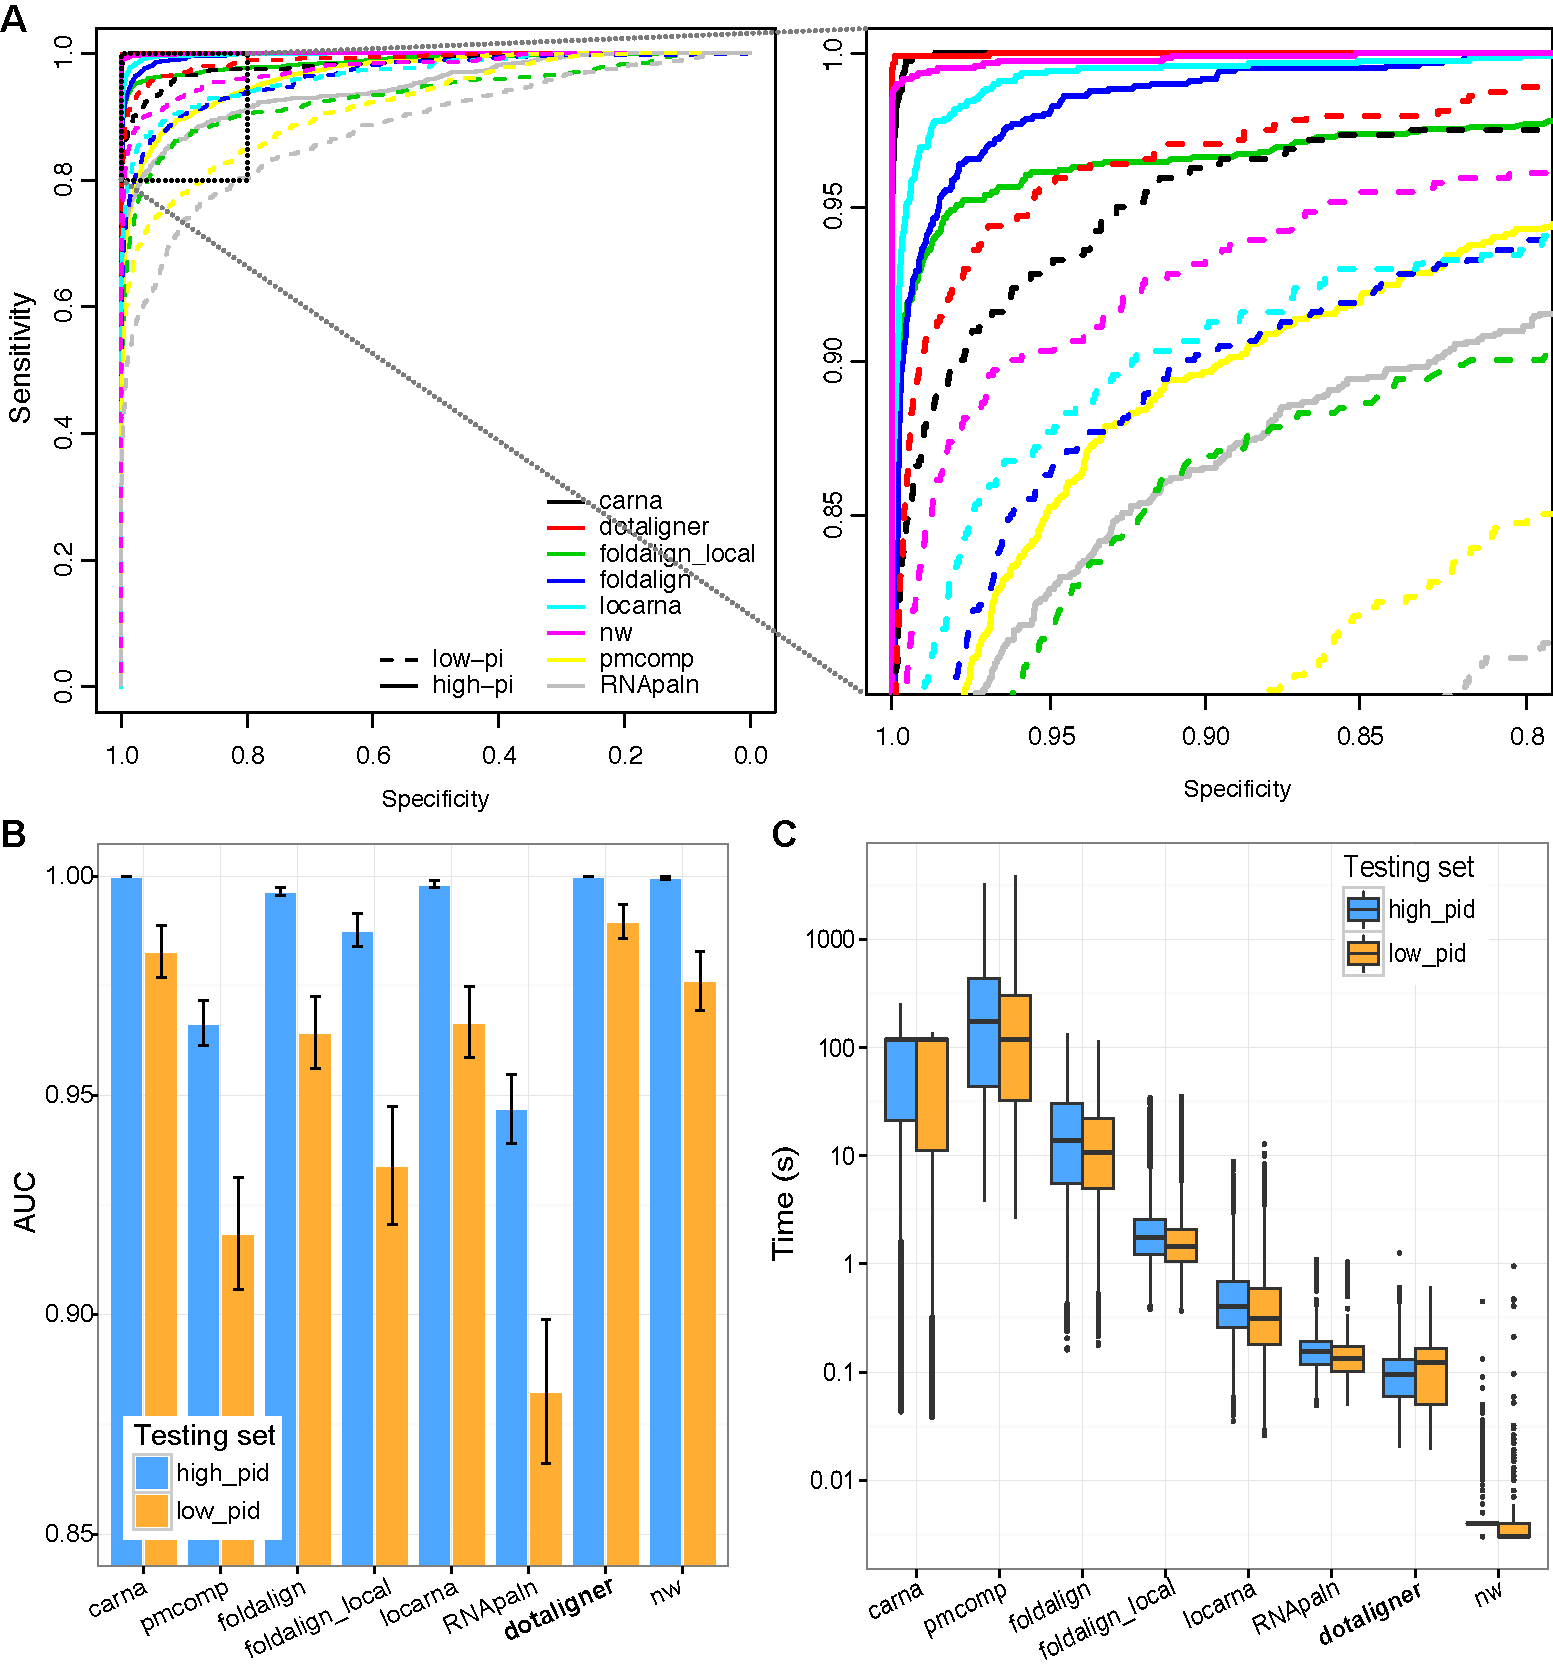
\includegraphics[width=\textwidth]{Fig2}
 \caption {\csentence{  
 Comparison of RNA structure alignment quality in function of sequence identity.}  
\bralibase{} reference RNA structure alignments were submitted to 5 different pairwise alignment algorithms, 
 including the Needleman-Wunsch sequence-only alignment algorithm. 
 \textbf{(Top)} The total number of surveyed alignments in function of pairwise sequence identity. The 
 Matthews Correlation Coefficient (MCC), difference in Structural Conservation Index ($\Delta$-SCI),
 and \texttt{RNAdistance} calculated topological edit distance between 
the \rnaalifold{} consensus of the computed alignment and the reference \bralibase{} alignment consensus 
 are compared in the lower 3 plots. 
 }
\end{figure}


%%%%%%%%%       FIGURE 3      %%%%%%%%%% 
\begin{figure}[h!]
%  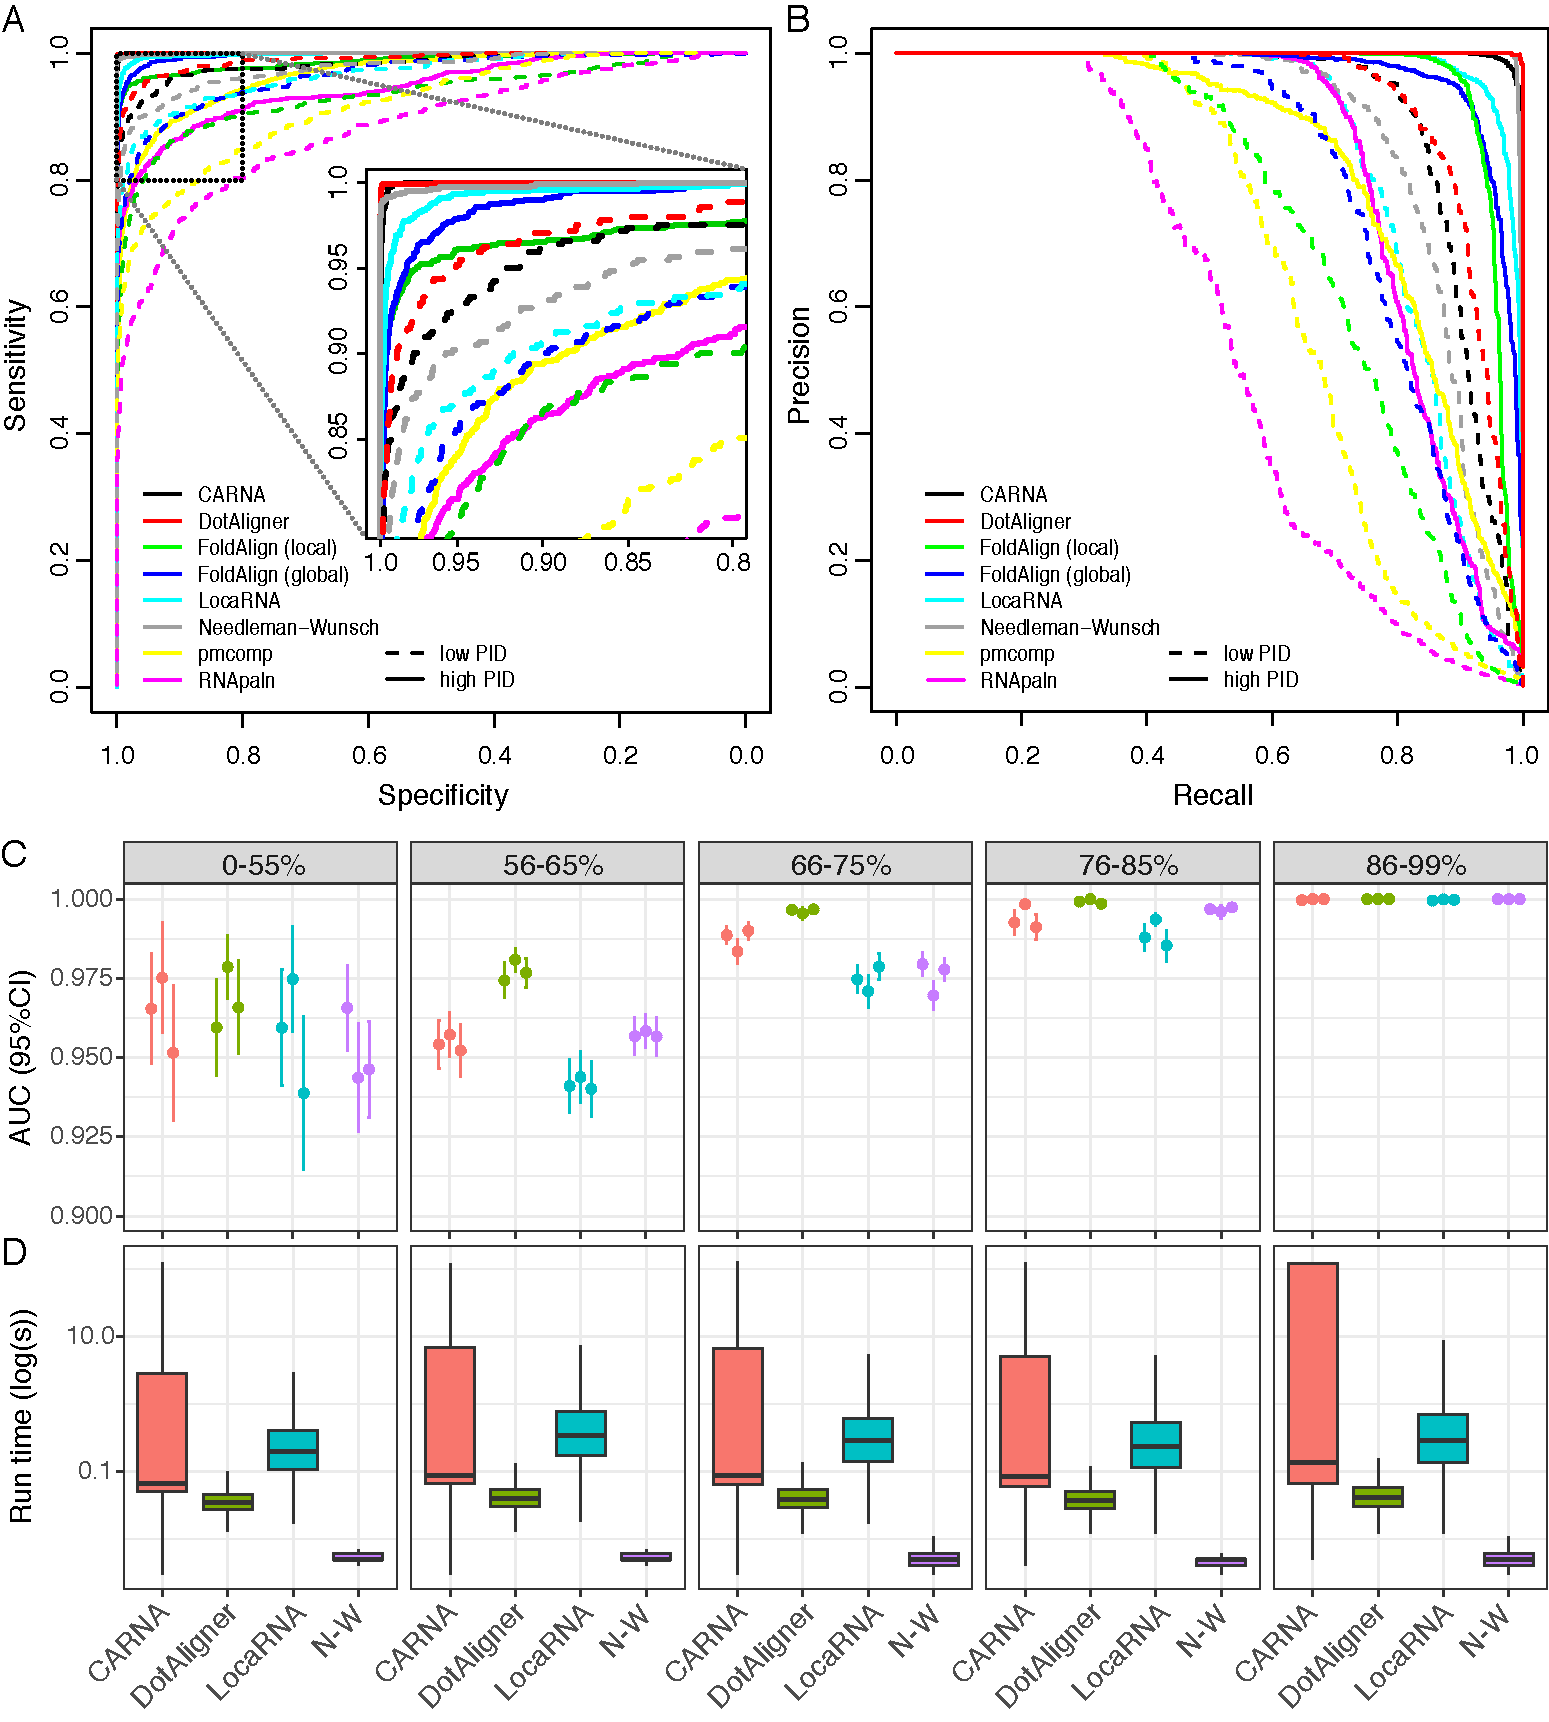
\includegraphics[width=\textwidth]{Fig3}
 \caption {\csentence{Classification of known RNA structures. }
 (\textbf{A}) Receiving Operator Characteristic (ROC) curves measuring the classification
 accuracy of surveyed algorithms by contrasting their computed similarity matrices 
 to a binary classification matrix of RFAM  sequences (1 if sequences are in same family; 
 0 if different). High PID =  56-95\% pairwise sequence identity from the provided RFAM alignment; Low PID  = 1-55\%.
 (\textbf{B}) Precision-recall curve;  
 (\textbf{C}) Area Under the Curve (AUC) of ROC values with 95\% confidence intervals 
for the top 4 performing algorithms across 5 ranges of pairwise sequence identity, 
 as calculated from a variant of the Needleman-Wunsch algorithm with free end gaps. 
 The 3 replicates correspond to stochastically sampled sequences from RFAM 12.3  (see Additional file 2: Table S1); 
 (\textbf{D}) Runtime distribution of single thread computation on a 2.6 GHz AMD Opteron processor 
 (N.B. a fixed upper limit of 120 s was  imposed for \carna{}). }  
\end{figure}


%%%%%%%%%       FIGURE 4      %%%%%%%%%% 
\begin{figure}[h!]
%  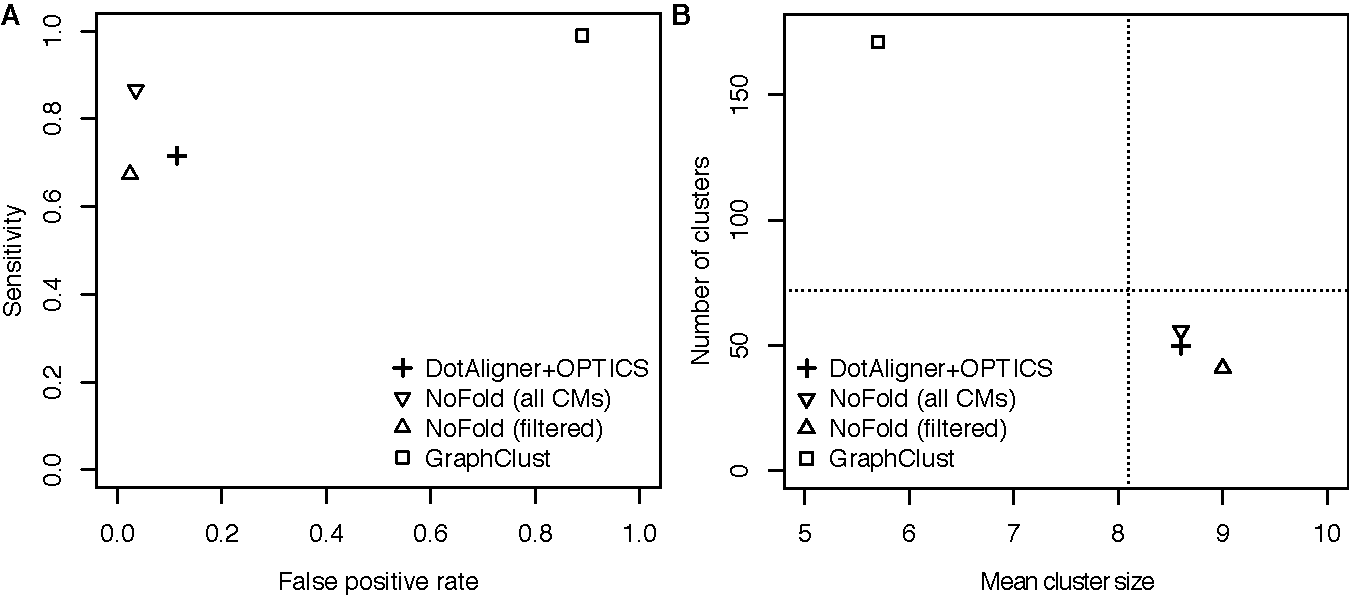
\includegraphics[width=\textwidth]{Fig4}
 \caption {\csentence{Comparative clustering benchmark of RFAM sequences and their shuffled controls}. Clustering performance metrics of 3 algorithms on 580 reference RFAM 
 structures and their dinucleotide-shuffled controls. (\textbf{A}) Sensitivity vs false positive rate; (\textbf{B}) Qualitative cluster statistics (horizontal dashed line indicate real amount of clusters from unique RFAM families). }
\end{figure}


%%%%%%%%%       FIGURE 5      %%%%%%%%%% 
\begin{figure}[h!]
%  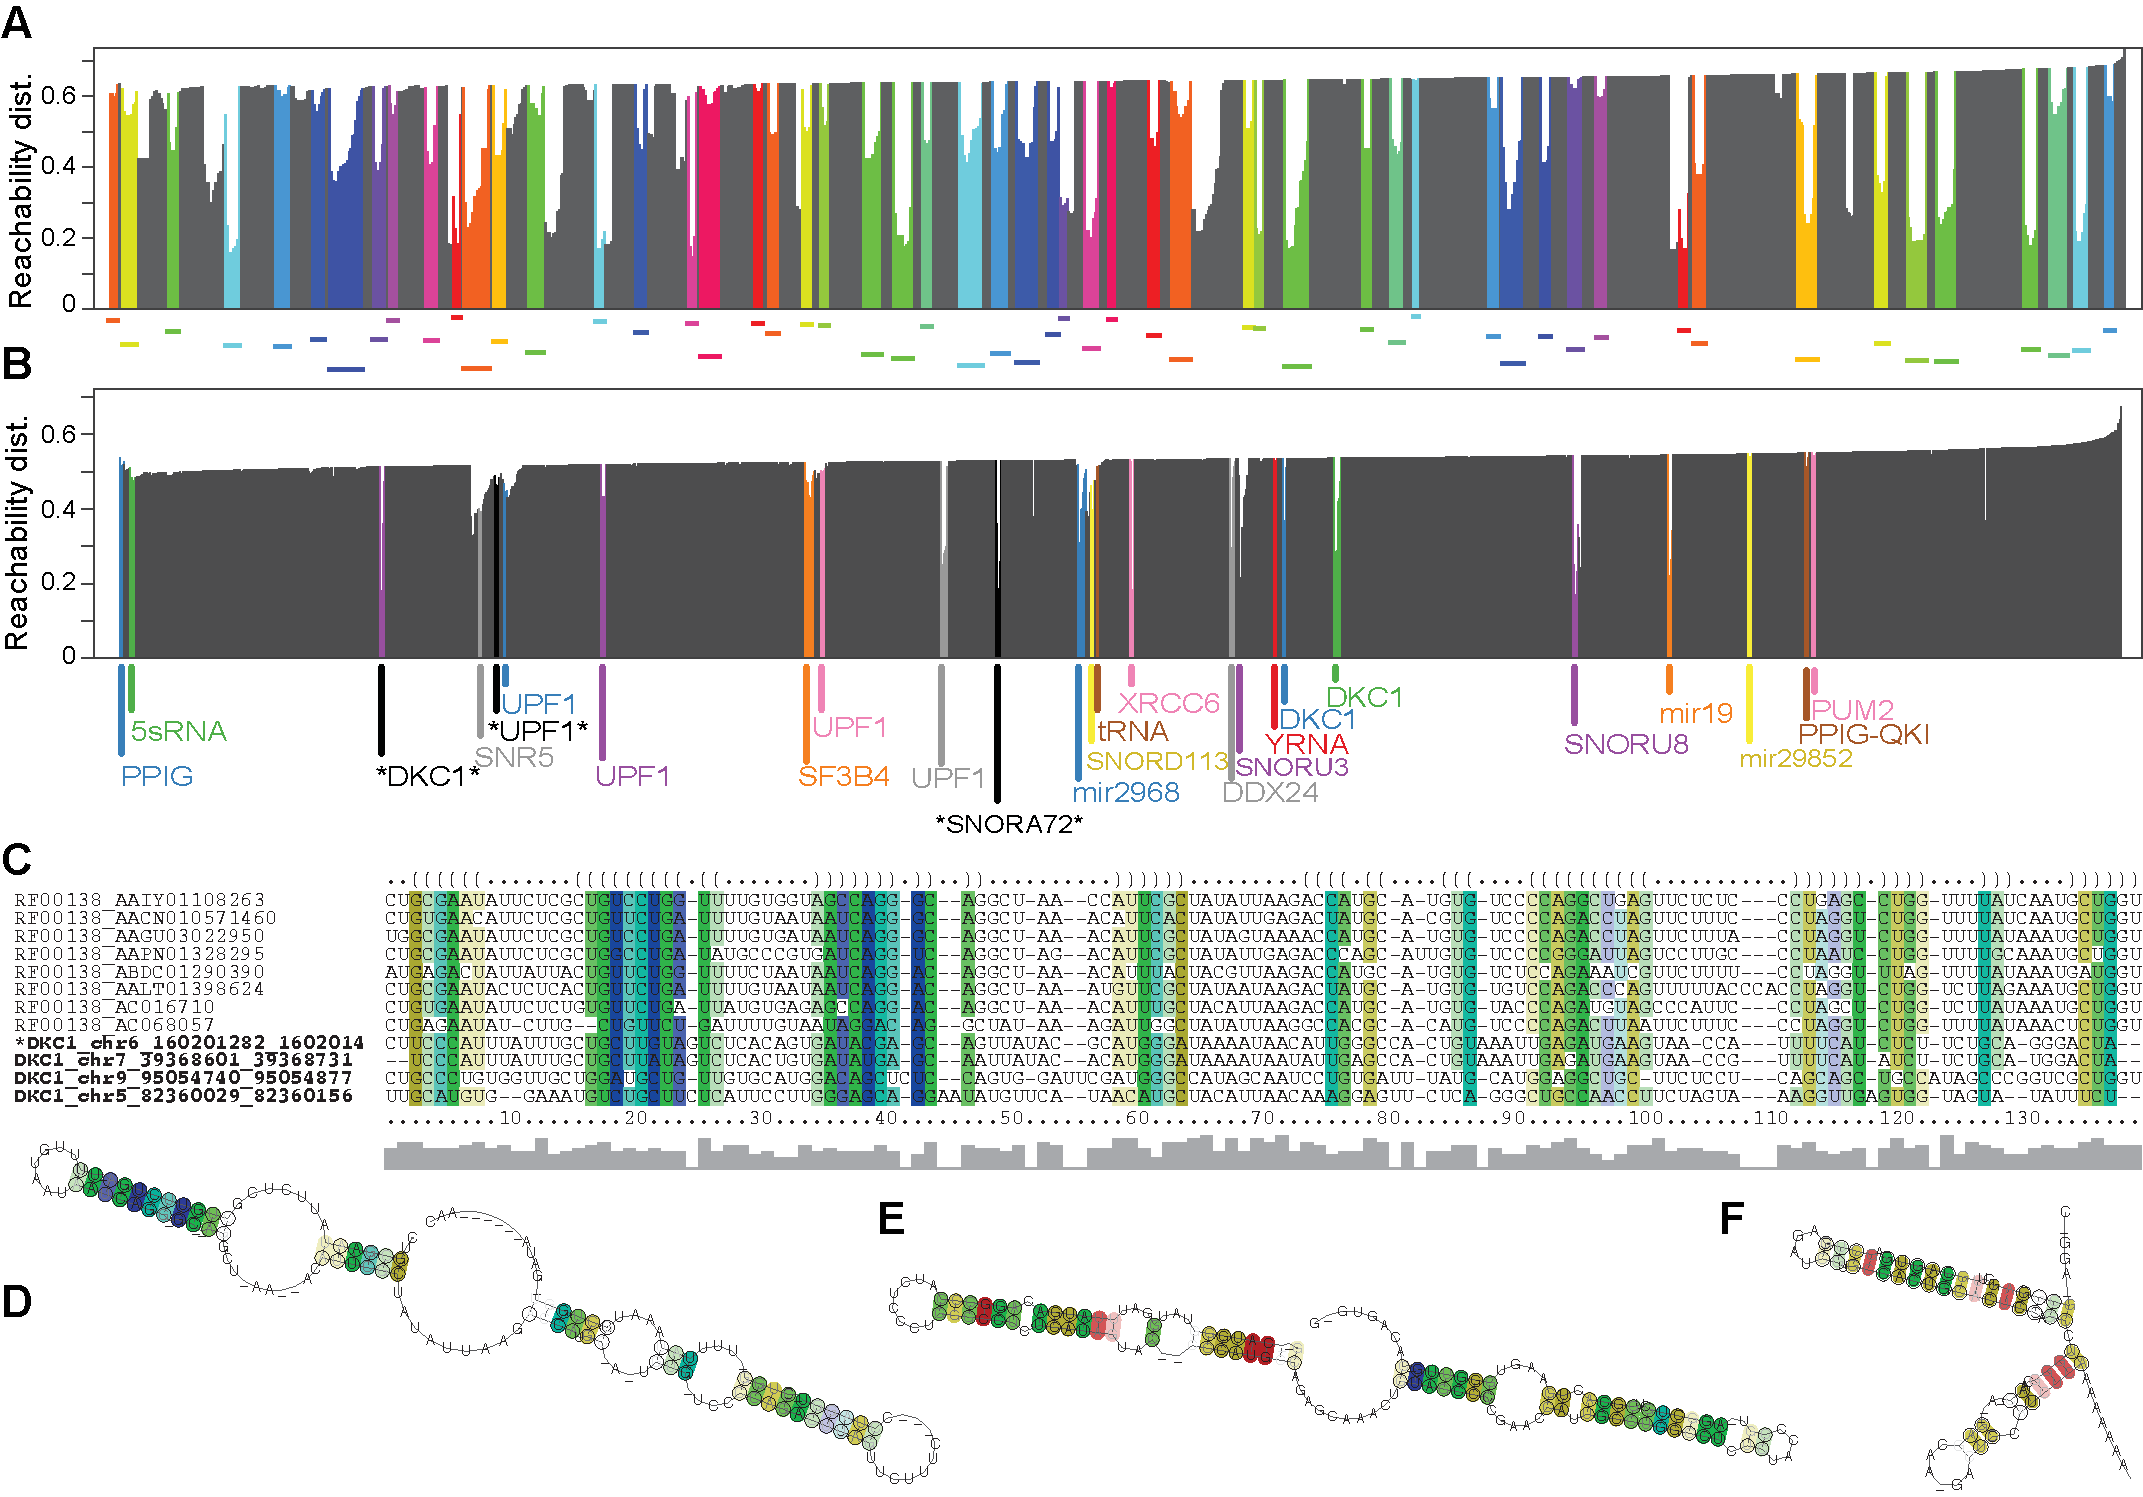
\includegraphics[width=\textwidth]{Fig5}
 \caption {\csentence{ De novo homologous RNA motif identification}. 
 (\textbf{A,B}) Reachability plots of OPTICS clustering display the OPTICS-derived ordering of points (x axis) and their distance to the nearest neighbour (y axis). Colours represent significant clusters: (\textbf{A}) Clustering of RFAM benchmarking data indicating the distance to the nearest neighbour,
 (\textbf{B}) Clustering of 2,650 ENCODE eCLIP peaks + 100 RFAM controls that overlap evolutionarily conserved secondary structure predictions. The dominant RNA binding protein in each cluster is displayed next to significant clusters; those with an asterisk are portrayed below.
 (\textbf{C}) Multiple structure alignment generated by \texttt{mLocaRNA} on the sequences from a 
 cluster containing both RFAM SNORNA72 sequences, and DKC1 (a snoRNA-binding protein) eCLIP peaks. 
An unannotated DKC1-bound sequence is marked with an asterix.
 (\textbf{D-F}) \texttt{RNAalifold} predicted consensus RNA secondary structures: 
 (\textbf{D}) Structure of the alignment displayed in (\textbf{C}), 
 (\textbf{E}) Structure of a cluster of impartially detected DKC1-bound snoRNAs, and
 (\textbf{F}) Structure of a novel UPF1-bound motif. }
\end{figure}


%%%%%%%%%%%%%%%%%%%%%%%%%%%%%%%%%%%
%%                               
%% Tables                        
%%                              

%% Use of \listoftables is discouraged.
%%
\section*{Tables}

%%%%%%%%%     TABLE 1    %%%%%%%%% 
\begin{table}[h!]
\caption{ Comparative clustering performance. }
 \begin{tabular}{ccccc}
 \hline
 Algorithm & \# Clusters & Sensitivity & Specificity & Accuracy \\
 \hline
 \dotaligner{}+\texttt{OPTICS} & 53 & 0.716 & 0.886& 0.802\\
 \texttt{GraphClust} & 201 & \textbf{0.990} & 0.110 & 0.635\\ % TN=78; FN=11
 \nofold{} (all CMs) & \textbf{62} & 0.866 & 0.965 & \textbf{0.916 }\\ % 
 \nofold{} (filtered) & 45 & 0.674 & \textbf{0.976} & 0.826\\ % TP=392;TN=575; FP=14;FN=190
 \hline
 \end{tabular}
\end{table}




%%%%%%%%%%%%%%%%%%%%%%%%%%%%%%%%%%%
%%                               
%% Additional Files       
%%                               
\section*{Additional files}

 \subsection*{Additional file 1 --- Supplementary methods}

 Link to GitHub repository, detailed description of the \dotaligner{} implementation, RNA structure clustering, and eCLIP data processing. 

 \subsection*{Additional file 2 --- Supplementary tables and figures}

\end{backmatter}

%%%%%%%%%%%%%%%%%%%%%%%%%%%%%%%%
%\newpage 
\clearpage

\section*{Additional file 1 --- Supplementary methods}
%%%%%%%%%%%%%%%%%%%%%%%%%%%%%%%%
The pipelines, scripts and some programs used in this work can be found in the 
GitHub repository associated to this work at \url{https://github.com/noncodo/BigRedButton}. 

\subsection*{ 1. \dotaligner{} implementation }
\noindent The weight $W$ of alignment \emph{A}
of two arc-annotated sequences $(S_a,P_a)$ and $(S_b,P_b)$ has been defined by \cite{Palu2010} as

\begin{equation}\label{eq1}
\begin{aligned}
	W(A) ={} & \sigma(A) + \tau(A) + \gamma(A) \\
	     ={} & \sum_{(i,i^\prime) \in A} \sigma(i,i^\prime) + \sum_{(i,j) \in
	P_a,\atop {(i^\prime,j^\prime) \in P_b,\atop {(i,i^\prime) \in
	A,\atop (j,j^\prime) \in A}}} \tau(i,j,i^\prime,j^\prime) + \gamma
	\times N
\end{aligned}
\end{equation}

\noindent where $S$ is a sequence and $P$ is a base pair probability matrix,
$\sigma(i,i^\prime)$ is the similarity of sequence positions $S_a[i]$ and
$S_b[i^\prime]$, $\tau(i,j,i^\prime,j^\prime)$ is the similarity of arcs $(i,j)
\in P_a$ and $(i^\prime,j^\prime) \in P_b$,
%$\tau(i,j,i^\prime,j^\primej,) = 1 - 2 \times |
%P_a(i,j)-P_b(i^\prime,j^\prime) |$)
and $\gamma$ is the gap cost associated with each sequence position that is not
matched ($N = |S_a|+|S_b|-2|A|$). The alignment problem finds the maximal
$W(A)$. As its solution is MAX-SNP-hard, in practise heuristics are used to find
near-optimal solutions.\\

\dotaligner{} solves the related problem of aligning two base pair
probability matrices (\emph{dot plots}). A major criteria for the implementation was a fast
running time enable all-vs-all pairwise structural alignments and the 
associated distance (dissimilarity) matrix, which can be used for 
cluster analysis of large data sets \cite{Will17432929}. Consequently, 
it employs a heuristic alignment-envelope, 
which imposes constraints to sub-optimal string alignments, 
and a fold-envelope, which imposes constraints to pre-calculated base pair probabilities, 
to build pairwise sequence-structure alignments. \\

Below, we describe the alignment procedure and weight functions.
The alignment procedure consists of two steps:
\begin{enumerate}
  \item Partition function of pairwise probabilistic string alignments; 
  \item Stochastic sampling of string alignments and scoring of aligned dot plots.
\end{enumerate}

\subsubsection*{1.1 Partition function of pairwise probabilistic string alignments}
In step 1 the computation of the partition function $Z(T)$ over all canonical pairwise
string alignments $A$ is adapted from probA \cite{Muckstein12385998}:

\begin{equation}\label{probA_Z}
	Z(T) = \sum_A exp( \beta W(A) ),
\end{equation}

\noindent where $\beta = 1/T$. Then the probability of a specific alignment $A$ is defined as:

\begin{equation}\label{probA}
	Pr(A;T) = \frac{1}{Z(T)} exp( \frac{W(A)}{T} ),
\end{equation}

\noindent The parameter $T$ is analogous to the temperature in the
thermodynamic interpretation of the alignment problem and determines the
relative importance of the optimal string alignment. If $T=1$ then we recover the
'true` probability, if $T\to0$ then $Pr(A;0)=0$ for all alignments with a score
$W(A)$ less then the score of the optimal string alignment, and if $T\to\infty$ then
all alignments have the same $Pr(A,\infty)=1/Z(\infty)$.  Hence, $T$ controls
the search space of suboptimal alignments for step 2. \textcolor{blue}{
The algorithm uses the dynamic programming algorithm of Gotoh \cite{Gotoh7166760} which has running time of $O(N^2)$.} 
The weight function $W(A)$ of
the probA implementation is changed to explore the ensemble of dot plot
alignments. We reduce the sequence-structure alignment problem to a
two-dimensional problem similar to the metric introduced in StrAL
\cite{Dalli16613908}. Hence, step 1 considers only the similarity $\sigma$ and
the gap cost $\gamma$ described in equation \ref{eq1}:

\begin{equation}\label{wstep1}
	W_{\mbox{Step1}}(A) = \sigma(A) + \gamma(A)
\end{equation}

\noindent The similarity $\sigma(i,i^\prime)$ for matched sequence positions $S_a[i]$ and
$S_b[i^\prime]$ takes into account sequence similarity $M_{Seq}$ and the
similarity in their unpaired probabilities $\Delta \omega(i,i^\prime)$ weighted
by the parameter $\theta$:

\begin{equation}\label{sigmam}
	\sigma(i,i^\prime) = \theta \times
		M_{Seq}^{(i,i^\prime)} + (1-\theta) \times \Delta \omega(i,i^\prime)
%	S_{Seq} = \sum_{(i,i^\prime) \in A} \tau \times M_{Seq}^{(i,i^\prime)} 
\end{equation}

\noindent  $M_{Seq}^{(i,i^\prime)}$ is 1 if sequence positions $S_a[i]$ and
$S_b[i^\prime]$ match and else 0. The similarity of unpaired probabilities is
defined as

\begin{equation}\label{eq3}
	\Delta \omega(i,i^\prime) \in \left\{ \begin{array}{cl}
			0 & \textrm{if } \omega(i) == 0 \\
			  & \textrm{and } \omega(i^\prime ) == 0 \\
			1 - | \omega(i) - \omega(i^\prime) | & \textrm{else}
		\end{array}\right.
\end{equation}

\noindent so that $\Delta \omega = (0,1)$. \\

The gap term in equation \ref{eq1} is replaced with affine gap costs:

\begin{equation}\label{eq6}
	\gamma(A) = l \times g_o + (N-l) \times g_{ext}
\end{equation}
	
\noindent where $l$ is the number of initiation gaps, $N$ is the number of all gaps,
$g_o$ is the penalty for opening a gap and $g_{ext}$ is the penalty for gap
extensions. Start and end gaps can be considered as free (set parameter \texttt{--free-endgaps}). \\

\subsubsection*{1.2 Stochastic sampling of string alignments and scoring of aligned dot plots}

Here, a properly weighted sample of stochastic pairwise string alignments
in the alignment ensemble is examined across both sequences for sequence-structure similarity.
The stochastic backtracking is adapted from probA \cite{Muckstein12385998} for
selecting $s$ suboptimal string alignments $A_s$.  The combined score (weight)
$W_{\mbox{Step2}}$ is a variant of equation \ref{eq1} to explore the similarity
of the corresponding dot plot alignments:

\begin{equation}\label{eq7}
	W_{\mbox{Step2}}(A_s) = \kappa \times \frac{W_{\mbox{Step1}}(A_s)}{|A_s|} + (1-\kappa) \times
	\frac{\tau(A_s)}{{|\mbox{Match}_{A_s}|}^2}
\end{equation}

\noindent where the parameter $\kappa$ weights for each alignment $A_s$ between the
sequence-based similarity $W_{\mbox{Step1}}(A_s)$ normalised by alignment
length $|A_s|$ and dot plot similarity $\tau(A_s)$ normalised by the number of
aligned bases $|\mbox{Match}_{A_s}|$ in alignment $A_s$. Similar to equation
\ref{sigmam} the dot plot similarity $\tau$ sums the parameter $\theta$ weighted
similarity of aligned base pairs $M_{paired}$ and the similarity in their
pairing probabilities $\Delta \psi$:

\begin{equation}\label{eq8}
	\tau(i,j,i^\prime,j^\prime) = \theta \times M_{paired}^{(i,j,i^\prime,j^\prime)}
	+ (1-\theta) \times \Delta \psi(i,j,i^\prime,j^\prime)
\end{equation}

\noindent where $M_{paired}^{(i,j,i^\prime,j^\prime)}$ is 1 if $S_a[i]$ and $S_a[j]$ as
well as $S_b[i^\prime]$ and $S_b[j^\prime]$ form canonical base pairs (G-C, C-G,
A-U, U-A, G-U or U-G) and else 0. The similarity in pairing probabilities
$\Delta \psi$ is then calculated by

\begin{equation}\label{eq9}
	\Delta \psi(i,j,i^\prime,j^\prime) \in \left\{ \begin{array}{l}
			0 \textrm{ if }\psi(i,j) == 0 
			  \textrm{ and }\psi(i^\prime,j^\prime) == 0 \\
		1 - | \psi(i,j) - \psi(i^\prime,j^\prime) | \textrm{ else}
		\end{array}\right.
\end{equation}

\noindent For both sequences $S_a$ and $S_b$, the pairing probability matrices $P_a$ and
$P_b$ are computed in advance using McCaskill's algorithm, implemented in
\texttt{RNAfold }or \texttt{RNAplfold}. The robustness of the alignment is improved by applying
log-odds scores $\psi$ of having a specific base pairing against the null model
of a random pairing \cite{Will17432929}:

\begin{equation}\label{eq11}
	\psi(i,j) = max \left( 0, log \frac{P(i,j)}{p_0} / log \frac{1}{p_0} \right)
\end{equation}

\noindent where $p_0$ is the expected probability for a pairing to occur at random. The
term $log \frac{1}{p_0}$ is a normalization factor that transforms the scores to
a maximum of 1. $P==1$ results in $\psi=1$, $P>p_0$ results in $\psi>0$, and $P\le
p_0$ results in $\psi=0$.  This transformation gives weaker similarities if low
base pair probabilities are compared, but stronger similarities for high base pair
probabilities. Unpaired probabilities are handled in a similar way by

\begin{equation}\label{eq12}
	\omega(i) = max \left( 0, log \frac{1 - \sum_k P(i,k)}{p_0} / log \frac{1}{p_0} \right)
\end{equation}

\noindent  where $p_0$ is the expected probability for an unpaired base to occur at
random.

\textcolor{blue}{
\subsubsection*{1.3 Alternative model using substitution rates}
}

Alternatively, the sequence and base pair similarities $M_{Seq}$ and $M_{paired}$ in equations \ref{sigmam} and \ref{eq8} can be replaced by the statistical substitution models $R_{Seq}$ and $R_{paired}$, respectively. In this (non-default) model of \dotaligner{} $R_{Seq}$ is multiplied with the $\zeta$
weighted sum of the similarity of unpaired probabilities $\Delta \omega$ and the similarity of upstream
pairing probabilities $\Delta \omega^{up}$ (set parameter \texttt{--mutation-rates}):

\begin{equation}\label{sigmar}
\begin{aligned}
	\sigma(i,i^\prime) ={} & R_{Seq}^{(i,i^\prime)} \times \zeta \times \Delta \omega(i,i^\prime) +  \\
			       & R_{Seq}^{(i,i^\prime)} \times (1-\zeta) \times
	\Delta \omega^{up}(i,i^\prime)
\end{aligned}
\end{equation}

\noindent  $R_{Seq}$ is a $4\times4$ matrix of probabilities for observing
a given substitution relative to background nucleotide frequencies. We use the
log-odd scores $L$ from the RIBOSUM85-60 matrix introduced in
\cite{Klein14499004} which are transformed to probabilities $R_{Seq}$ by
$2^{L(i,i^\prime)} / (1 + 2^{L(i,i^\prime)})$. The ratio of upstream pairing probability
$\omega^{up}$ is defined as

\begin{equation}\label{eq5}
	\omega^{up}(i) = \sum_{k=1}^{i-1} \psi(k,i) /
	\sum_{k=1}^{|S|} \psi(k,i)
\end{equation}

\noindent where $i \in S$, $|S|$ is the length of sequence $S$, and $\psi(k,i)$ is the
pairing probability of sequence positions $S[k]$ and $S[i]$. The downstream
pairing probability is implicitly considered in the weight function through the
usage of unpaired probability and upstream pairing probability.

\noindent The base pair similarity matrix
$M_{paired}$ can be replaced by a statistical substitution model $R_{paired}$
which describes the probability for observing a given base pair substitution
relative to background nucleotide frequencies:

\begin{equation}\label{eq10}
	\tau(i,j,i^\prime,j^\prime) = R_{paired}^{(i,j,i^\prime,j^\prime)}
\times \Delta \psi(i,j,i^\prime,j^\prime)
\end{equation}

\noindent The log-odd scores $L$ from the RIBOSUM85-60 matrix \cite{Klein14499004}
	are transformed to probabilities $R_{paired}$ by $2^{L(i,j,i^\prime,j^\prime)} / (1 + 2^{L(i,j,i^\prime,j^\prime)})$.\\


\subsection*{ 2. Clustering RNA structures with randomised controls }

Below is the code used to calculate the accuracy and other performance metrics of 
the clustering benchmark of stochastically sampled RFAM entries. All files can be found on the 
associated \texttt{GitHub} repository \url{https://github.com/noncodo/BigRedButton}.

\lstinputlisting{../data/clustering_benchmark/eval_acc.R}


\subsection*{ 3. eCLIP data processing }
Data in .bigBed format was acquired from the ENCODE data hub from the following link:
\url{https://www.encodeproject.org/search/?type=Experiment&assay_term_name=eCLIP&files.file_type=bigBed+narrowPeak&month_released=April\%2C+2016}

\begin{lstlisting}
#!/bin/bash

# Convert accessions to protein IDs
cut -f 1,16,29 metadata.tsv | sed 's/-human /_/g' | while read line 
do 
  F1=$(echo $line | awk '{print $1".bed"}' ) 
  F2=$( echo $line | awk '{ print $2".bed"}') 
  cp $F1 $F2 
done 

# Rename files accordingly
for file in *bed
do 
  mv $file $(head -n 1 $file | cut -f 4).bed
done

# Filter for greater than or equal to 8x fold enrichment
# And -log10( P-value ) greater than or equal to  4
for file in *rep0?.bed 
do
  awk '{if ($7 >= 4 && $8 >= 4) print }' $file > ../filtering/${file}_filt3
done

#Intersect both replicates (>1 overlap) 
for file in *rep01.bed_filt3 ; do     
    >&2 echo "Processing "$file
    bedtools intersect -s -u -f 0.5 -a <( cut -f 1-6 $file ) -b <( cut -f 1-6 ${file//rep01/rep02} )  > ${file}_1
    bedtools intersect -s -u -f 0.5 -b <( cut -f 1-6 $file ) -a <( cut -f 1-6 ${file//rep01/rep02} )  > ${file}_2
    
    # merge peaks if they are close together
    bedtools merge -d 50 -s -delim "|" -c 4,5,6 -o first,count,first -i <( cat ${file}_1 ${file}_2  | sort -k 1,1 -k 2,2n ) > ${file%*.bed_filt3}_filt_0.5_merged_50_s.bed
    
   # intersect with ECS (in file ECS_congruous_sorted.bed6) 
    bedtools intersect -wo -s -b ${file%*.bed_filt3}_filt_0.5_merged_50_s.bed -a ECS_congruous_sorted.bed6 > ${file%*.bed_filt3}_filt_0.5_merged_50_s_anyECS.bed
done

#merge all files into one
cat *_50_s_anyECS_merged.bed > All_ECS_merged_50nt_peaks.bed
# wc -l  All_ECS_merged_50nt_peaks.bed
## 2650

#edit sequence names and get sequence from reference genome (hg19) 
awk 'OFS="\t"{print $1,$2,$3,$4"_"$1"_"$2"_"$3"_"$6,$5,$6}'  ./All_ECS_merged_50nt_peaks.bed > ./All_ECS_merged_50nt_peaks_renamed.bed
bedtools getfasta -s -name -fi ~/data/fasta/hg19.fa -bed ./All_ECS_merged_50nt_peaks_renamed.bed -fo ./All_ECS_merged_50nt_peaks_renamed.fasta

#combine with known control RNA structure
cat All_ECS_merged_50nt_peaks_renamed.fasta spike-ins.fasta > All_ECS_merged_50nt_peaks_renamed_spikeIns.fasta
\end{lstlisting}

%%
%% TABLES
%%
%\begin{table}
%\centering
%\caption{Supplementary Table X: }
%\medskip
%\begin{tabular}{ccccc}
%\hline
%Params 	low_PI rank 	high_PI rank 	merged rank 	Low AUC 	High AUC 	AUC sum 	Low time 	High Time 	Combined 	low time stdev 	high time stdev 
%T-10_s-1_k- 0.3_t-0.5_o- 1_e-0.05.dot aligner.score .short 	1	112	112	0.98329790 3 	0.99617899 4 	1.97948	0.06335920 4 	0.07691424 1 	0.140273	0.04164723	0.04868907 5 
%T-1_s-1_k-0. 3_t-0.8_o-1_ e-0.05.dotali gner.score.s hort 	181	1	181	0.95934248 9 	0.99718898 5 	1.95653	0.06386044 8 	0.06963538 7 	0.133496	0.04032855 5 	0.05003469 8 
%T-1_s-1_k-0. 3_t-0.5_o-1_ e-0.05.dotali gner.score.s hort 	2	110	220	0.98329790 3 	0.99617899 4 	1.97948	0.06399656 7 	0.07126550 4 	0.135262	0.04146411 1 	0.04598433 1 
%T-5_s-1_k-0. 3_t-0.5_o-1_ e-0.05.dotali gner.score.s hort 	3	109	327	0.98329790 3 	0.99617899 4 	1.97948	0.06506572 1 	0.06912250 6 	0.134188	0.04589721 5 	0.04647907 1 
%T-10_s-5_k- 0.3_t-0.8_o- 1_e-0.05.dot aligner.score .short 	184	2	368	0.95934248 9 	0.99718898 5 	1.95653	0.06980044 8 	0.07476498 7 	0.144565	0.04664177	0.04667025 8 
%T-1_s-5_k-0. 3_t-0.5_o-1_ e-0.05.dotali gner.score.s hort 	4	113	452	0.98329790 3 	0.99617899 4 	1.97948	0.07141248 8 	0.07887591 7 	0.150288	0.04276297 3 	0.05162383 7 
%T-10_s-1_k- 0.3_t-0.8_o- 1_e-0.05.dot aligner.score .short 	182	3	546	0.95934248 9 	0.99718898 5 	1.95653	0.0654999	0.07663676 7 	0.142137	0.04187294 9 	0.04867886 9 

%\begin{table}
%\centering
%\caption{This is a table with scientific results.}
%\medskip
%\begin{tabular}{ccccc}
%\hline
%1 & 2 & 3 & 4 & 5\\
%\hline
%aaa & bbb & ccc & ddd & eee\\
%aaaa & bbbb & cccc & dddd & eeee\\
%aaaaa & bbbbb & ccccc & ddddd & eeeee\\
%aaaaaa & bbbbbb & cccccc & dddddd & eeeeee\\
%1.000 & 2.000 & 3.000 & 4.000 & 5.000\\
%\hline
%\end{tabular}
%\end{table}

\newpage

\section*{Additional file 2 --- Supplementary Tables and Figures}

\begin{table}[h]
\caption*{\textbf{Table S1.} Uniqueness and diversity of stochastically sampled RFAM subsets }
\begin{tabular}{cccccc}
\hline
 & & & \multicolumn{3} {c} { \# RFAM families }\\
 \cline{4-6}
Pairwise identity range & \# sequences & \% unique & Rep. 1  & Rep. 2 & Rep. 3 \\
\hline
0-55 &  178 & 94.4 & 33 & 19 & 32 \\
56-65 & 900 & 92.2 & 113 & 108 & 110 \\  
66-75 & 899 & 92.6 & 83 & 76 & 74   \\
76-85 &  900 & 91.7 & 80 & 82 & 79  \\
86-99 &  900 & 93.6 & 58 & 47 & 59 \\
\hline
\end{tabular}
\end{table}

\begin{table}
\centering
\caption*{\textbf{Table S2.}  List of RFAM families from benchmark that did not cluster}
\begin{tabular}{cll}
\hline
Sequence count & RFAM ID & RFAM family \\
\hline
2 & RF00005 &  tRNA \\
5 & RF00015 &  U4 spliceosomal RNA \\
8 & RF00020 &  U5 spliceosomal RNA \\
5 & RF00021 &  Spot 42 RNA \\
1 & RF00026 &  U6 spliceosomal RNA \\
10 & RF00059 &  TPP riboswitch (THI element) \\
5 & RF00167 &  Purine riboswitch \\
11 & RF00169 &  Bacterial small signal recognition particle RNA \\
13 & RF00199 &  SL2 RNA \\
4 & RF00374 &  Gammaretrovirus core encapsidation signal \\
11 & RF00378 &  Qrr RNA \\
6 & RF00386 &  Enterovirus 5' cloverleaf cis-acting replication element \\
6 & RF00389 &  Bamboo mosaic virus satellite RNA cis-regulatory element \\
4 & RF00444 &  PrrF RNA \\
17 & RF00494 &  Small nucleolar RNA U2-19 \\
2 & RF00515 &  PyrR binding site \\
4 & RF00550 &  Hepatitis E virus cis-reactive element \\
7 & RF01685 &  6S-Flavo RNA \\
7 & RF01697 &  Chlorobi-RRM RNA \\
6 & RF01705 &  Flavo-1 RNA \\
4 & RF01725 &  SAM-I/IV variant riboswitch \\
2 & RF01728 &  STAXI RNA \\
7 & RF01734 &  crcB RNA \\
1 & RF01750 &  pfl RNA \\
6 & RF01754 &  radC RNA \\
4 & RF01764 &  yjdF RNA \\
5 & RF02033 &  HNH endonuclease-associated RNA and ORF (HEARO) RNA \\
\hline
\end{tabular}
\end{table}

\begin{table}
\centering
\caption*{\textbf{Table S3.}  List of control RNA structures }
\begin{tabular}{ccc}
\hline
Sequences & RNA family & RFAM ID \\
\hline
   5 & 5SRNA & RF00002 \\
   8 & SNORA72 & RF00138 \\
  10 & SNORD113 & RF00181\\
  10 & SNORU3 & RF00012\\
  10 & SNORU8 & RF00096\\
   8 & SNR5 & RF01252\\
   9 & YRNA & RF00019\\
  10 & mir19 & RF00245\\
   7 & mir2968 & RF02093\\
   6 & mir29852 & RF02095\\
  17 & tRNA & RF00005\\
\hline
\end{tabular}
\end{table}

\begin{table}
\caption*{\textbf{Table S4.} Rank-product of best \dotaligner{} parameters}
\resizebox{\textwidth}{!}{\begin{tabular}{lccccccc}
\hline
Parameters  & low\_PI rank & high\_PI rank & rank product & low\_PI AUC & high\_PI AUC & AUC  sum  & Combined Time  \\
\hline
k=0.3 t=0.5 o=1 e=0.05 & 1 & 112 & 112 & 0.983297903 & 0.996178994 & 1.97948 & 0.140273\\
k=0.3 t=0.8 o=1 e=0.05 & 181 & 1 & 181 & 0.959342489 & 0.997188985 & 1.95653 & 0.133496\\
k=0.3 t=0.5 o=1 e=0.05 & 2 & 110 & 220 & 0.983297903 & 0.996178994 & 1.97948 & 0.135262\\
k=0.3 t=0.5 o=1 e=0.05 & 3 & 109 & 327 & 0.983297903 & 0.996178994 & 1.97948 & 0.134188\\
k=0.3 t=0.8 o=1 e=0.05 & 184 & 2 & 368 & 0.959342489 & 0.997188985 & 1.95653 & 0.144565\\
k=0.3 t=0.5 o=1 e=0.05 & 4 & 113 & 452 & 0.983297903 & 0.996178994 & 1.97948 & 0.150288\\
k=0.3 t=0.8 o=1 e=0.05 & 182 & 3 & 546 & 0.959342489 & 0.997188985 & 1.95653 & 0.142137\\
k=0.3 t=0.5 o=1 e=0.05 & 5 & 114 & 570 & 0.983297903 & 0.996178994 & 1.97948 & 0.156738\\
k=0.3 t=0.5 o=1 e=0.05 & 6 & 111 & 666 & 0.983297903 & 0.996178994 & 1.97948 & 0.155101\\
k=0.3 t=0.8 o=1 e=0.05 & 185 & 4 & 740 & 0.959342489 & 0.997188985 & 1.95653 & 0.146729\\
k=0.3 t=0.5 o=1 e=0.05 & 7 & 115 & 805 & 0.983297903 & 0.996178994 & 1.97948 & 0.186257\\
k=0.3 t=0.5 o=1 e=0.05 & 8 & 116 & 928 & 0.983297903 & 0.996178994 & 1.97948 & 0.192388\\
k=0.3 t=0.8 o=1 e=0.05 & 186 & 5 & 930 & 0.959342489 & 0.997188985 & 1.95653 & 0.154183\\
k=0.3 t=0.5 o=1 e=0.05 & 9 & 117 & 1053 & 0.983297903 & 0.996178994 & 1.97948 & 0.210514\\
k=0.3 t=0.8 o=1 e=0.05 & 183 & 6 & 1098 & 0.959342489 & 0.997188985 & 1.95653 & 0.154234\\
k=0.3 t=0.5 o=1 e=0.05 & 10 & 119 & 1190 & 0.983297903 & 0.996178994 & 1.97948 & 0.285647\\
k=0.4 t=0.6 o=1 e=0.05 & 13 & 97 & 1261 & 0.983273039 & 0.996343919 & 1.97962 & 0.133738\\
k=0.3 t=0.5 o=1 e=0.05 & 11 & 118 & 1298 & 0.983297903 & 0.996178994 & 1.97948 & 0.269801\\
k=0.3 t=0.8 o=1 e=0.05 & 187 & 7 & 1309 & 0.959342489 & 0.997188985 & 1.95653 & 0.187293\\
k=0.4 t=0.6 o=1 e=0.05 & 14 & 101 & 1414 & 0.983273039 & 0.996343919 & 1.97962 & 0.144514\\
\hline
\end{tabular}}
\end{table}

\begin{figure}
 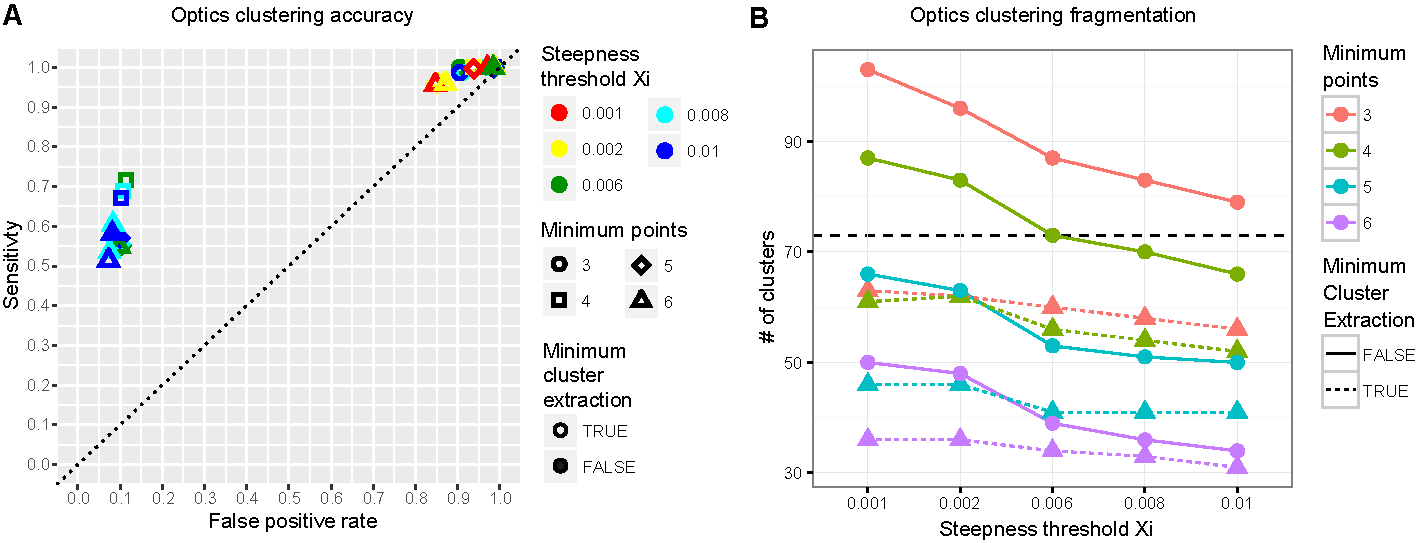
\includegraphics[width=0.45\textwidth]{SF1}
 \caption*{ \textbf{ Figure S1. Pairwise alignments of dot plots of SAM riboswitch. }\\
 The two sequences AM420293\_1 (upper triangles of the dot plots) and CP000580\_2\_6 (lower triangles) of the 5S-adenosyl methionine (SAM) riboswitch (Rfam family RF00634) are aligned (\textbf{A}) as in the Rfam reference alignment, (\textbf{B}) through \dotaligner's pairwise probabilistic string alignment (step 1), and (\textbf{C}) through \dotaligner's sampling of stochastic alignments (step 2). \dotaligner's sampling increases the combined score of the alignment from 0.58 to 0.60 (and the sequence identity from 56\% to 63\%), and improves the quality of the alignment compared to the Rfam reference.
}
\end{figure}

\begin{figure}
 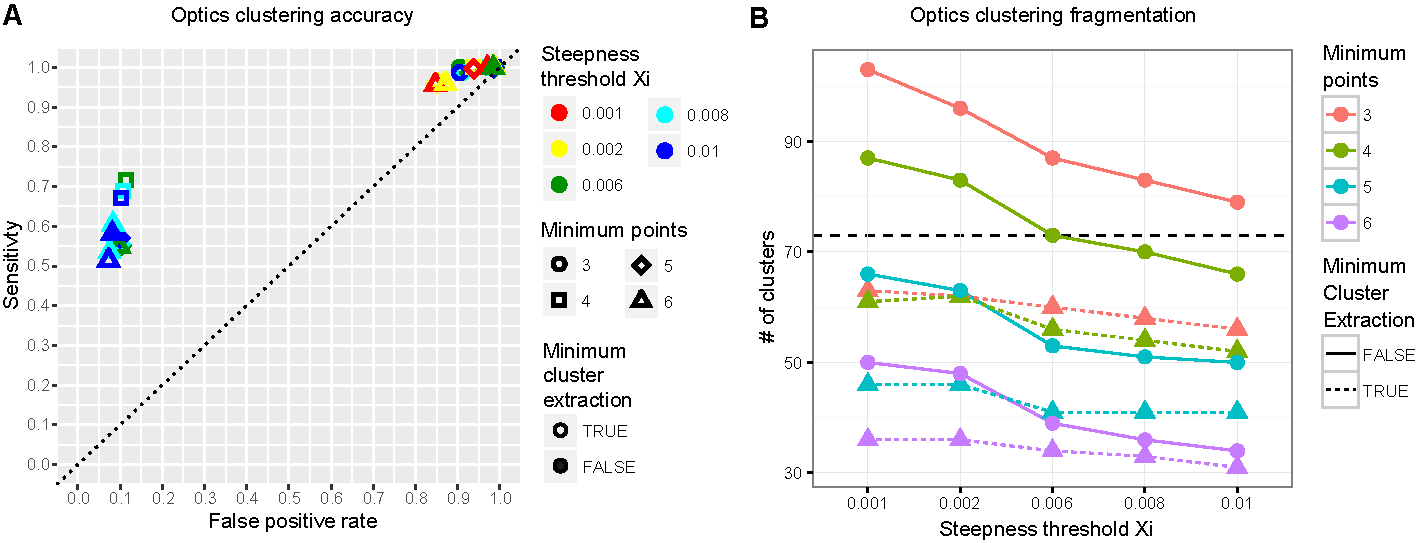
\includegraphics[width=\textwidth]{SF2}
 \caption*{ \textbf{ Figure S2. Impact of sampling of stochastic alignments on the alignment score.}\\
	We executed \dotaligner{} (default runtime parameters) while (\textbf{A}) varying parameter $T$ (sampling diversity) with 1000 samples (parameter $s$) and (\textbf{B}) varying the number of samples with $T=0.25$ on the RFAM binary classification benchmark datasets corresponding to 0-55\% and 56-65\% sequence identity (PID) (3 replicates each). For parameter $T$ equal 0.1 and 0.25 the majority of pairwise alignments are optimized through the sampling procedure (sample increased the alignment score) (\textbf{A}). In few cases, $T$=0.5 also produced an optimized alignment through sampling. In average the alignment score saturates after 1000 samples of the stochastic backtracking for $T=0.25$ (\textbf{B}).
}
\end{figure}

\begin{sidewaysfigure}
    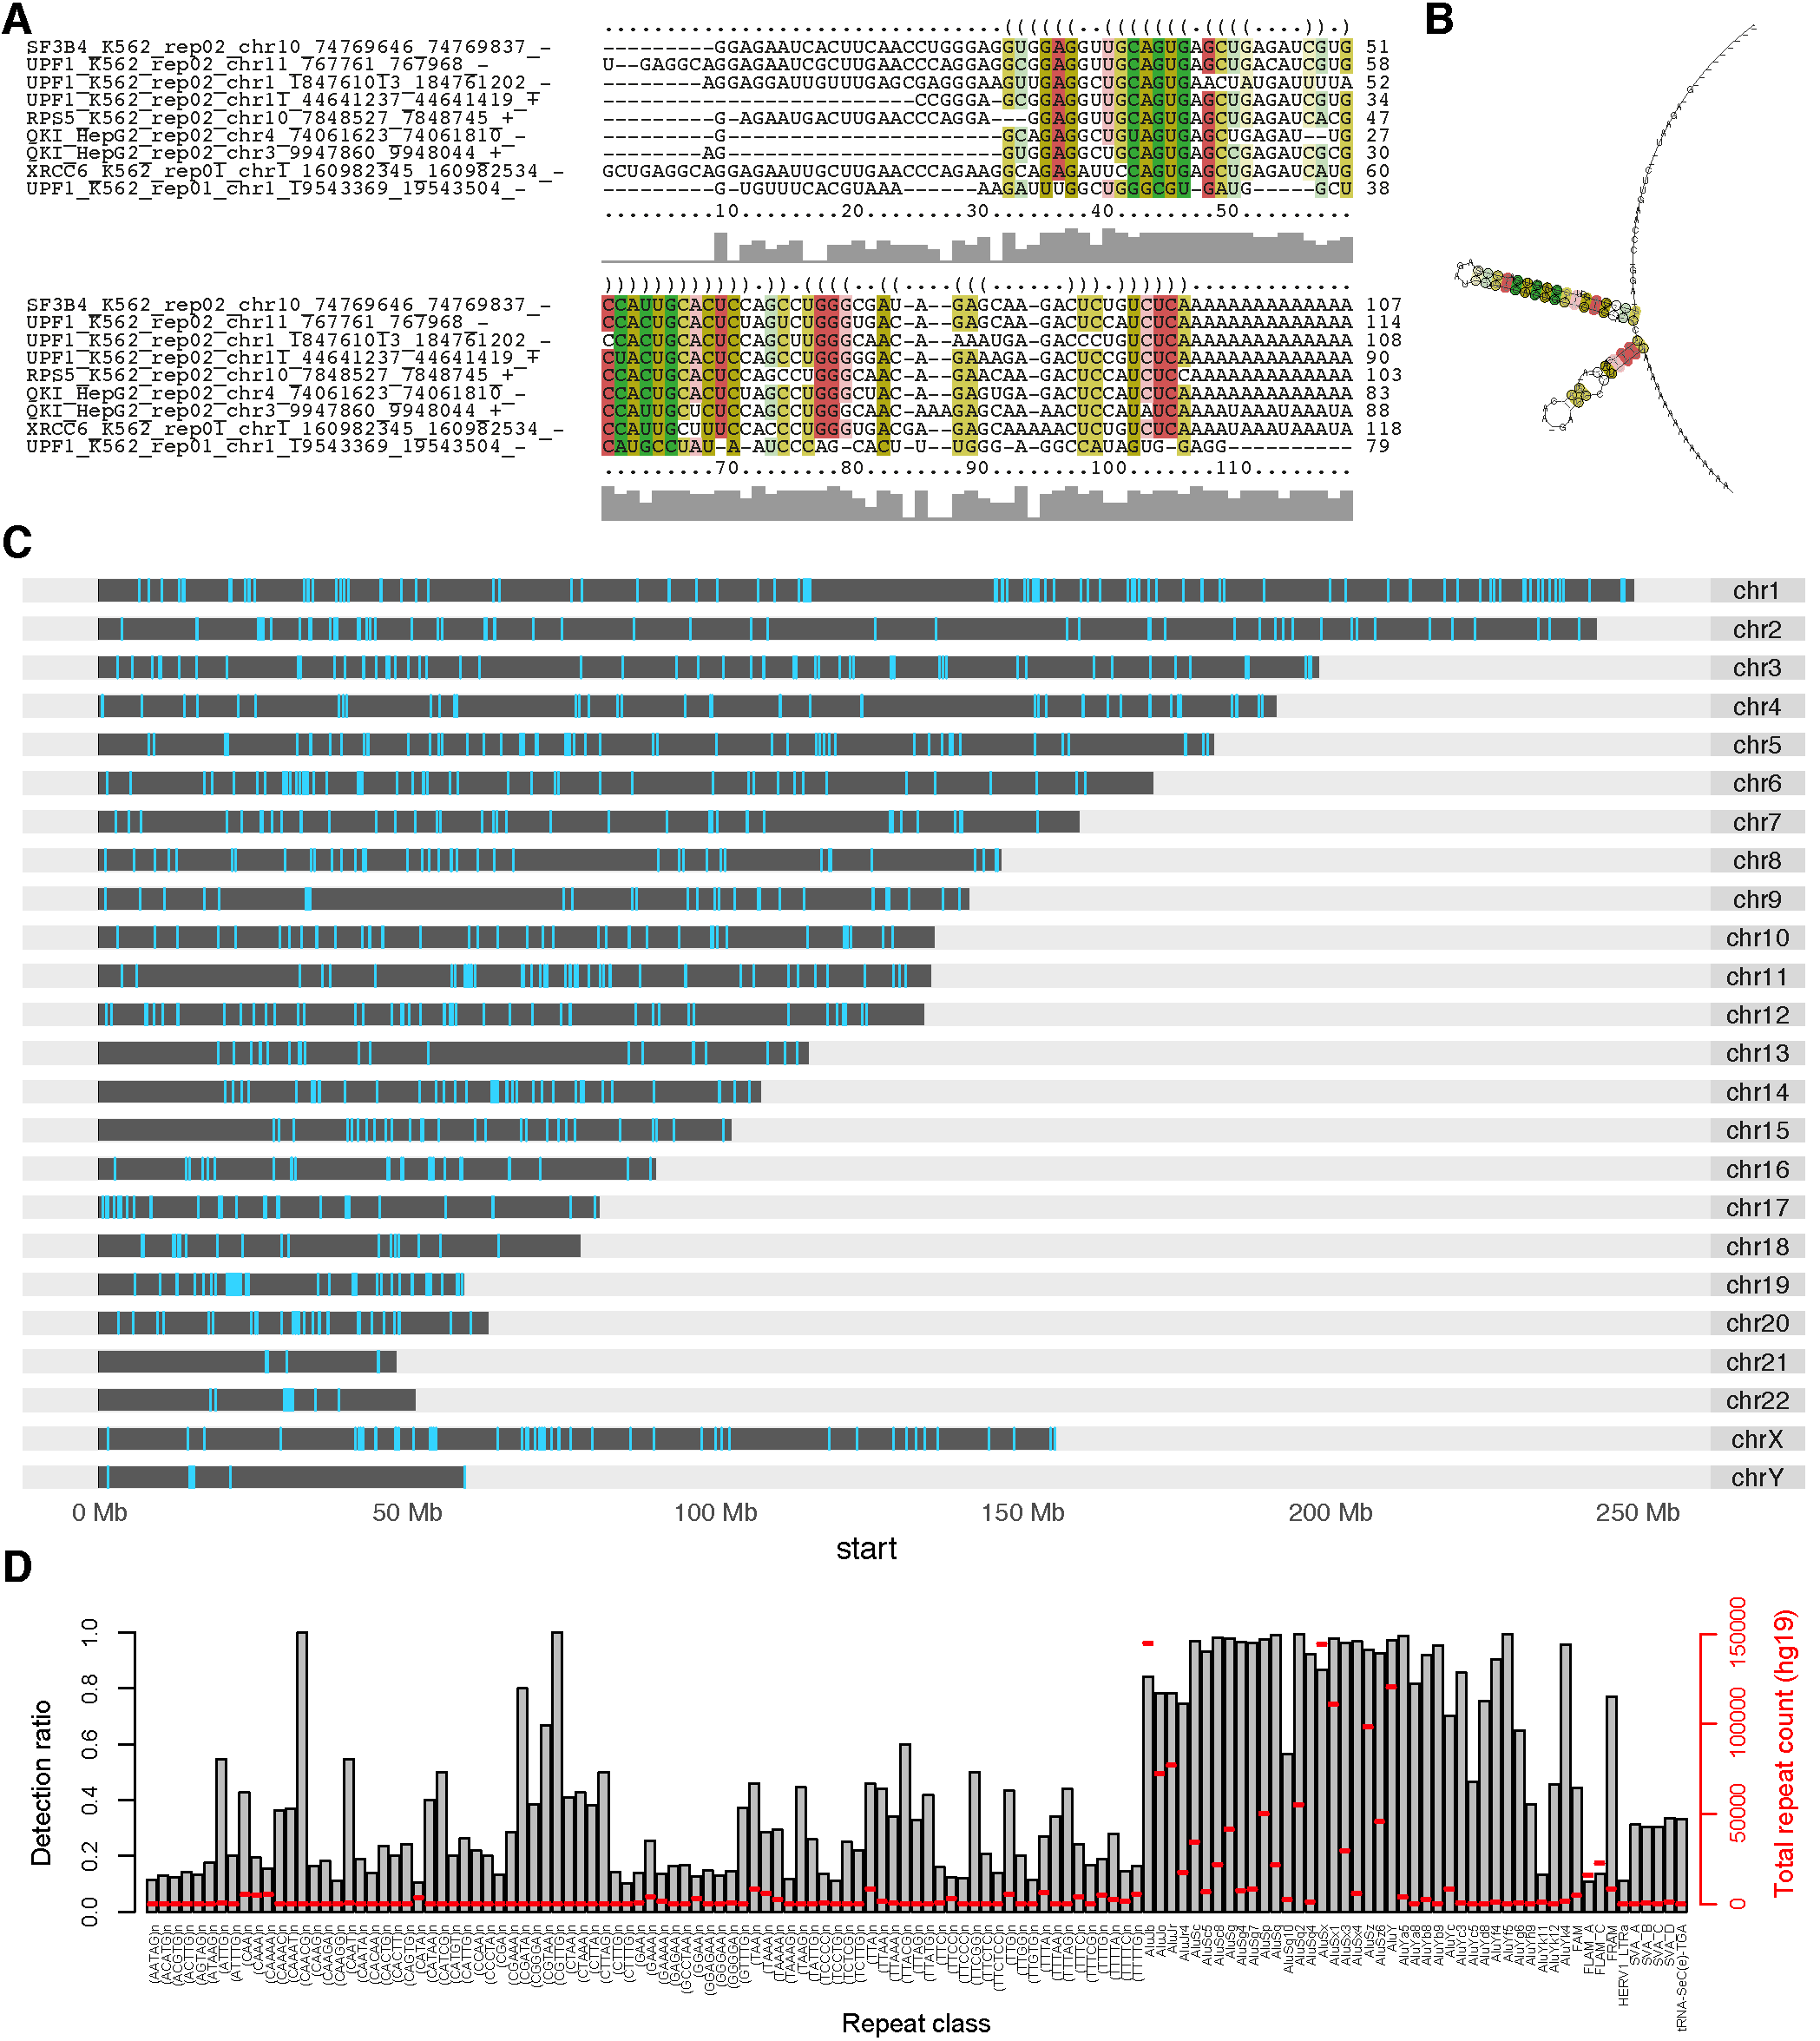
\includegraphics[width=\textwidth]{SF3}
     \caption*{ \textbf{ Figure S3. Binary classification of similarity matrices  }\\
Stochastically sampled RFAM version 12.0 sequences are labelled as belonging to the same family in white, and in red when not (Left). Heat maps of the similarity matrices produced by \dotaligner{}, \locarna{} and \carna{} are listed in columns 2, 3 and 4, respectively.  
(top) Low mean pairwise identity samples, where each sequence within 
a family shares between 0 and 55\% sequence identity; (bottom) Higher (56-95\%) mean pairwise identity samples. }
\end{sidewaysfigure}


\begin{figure}
 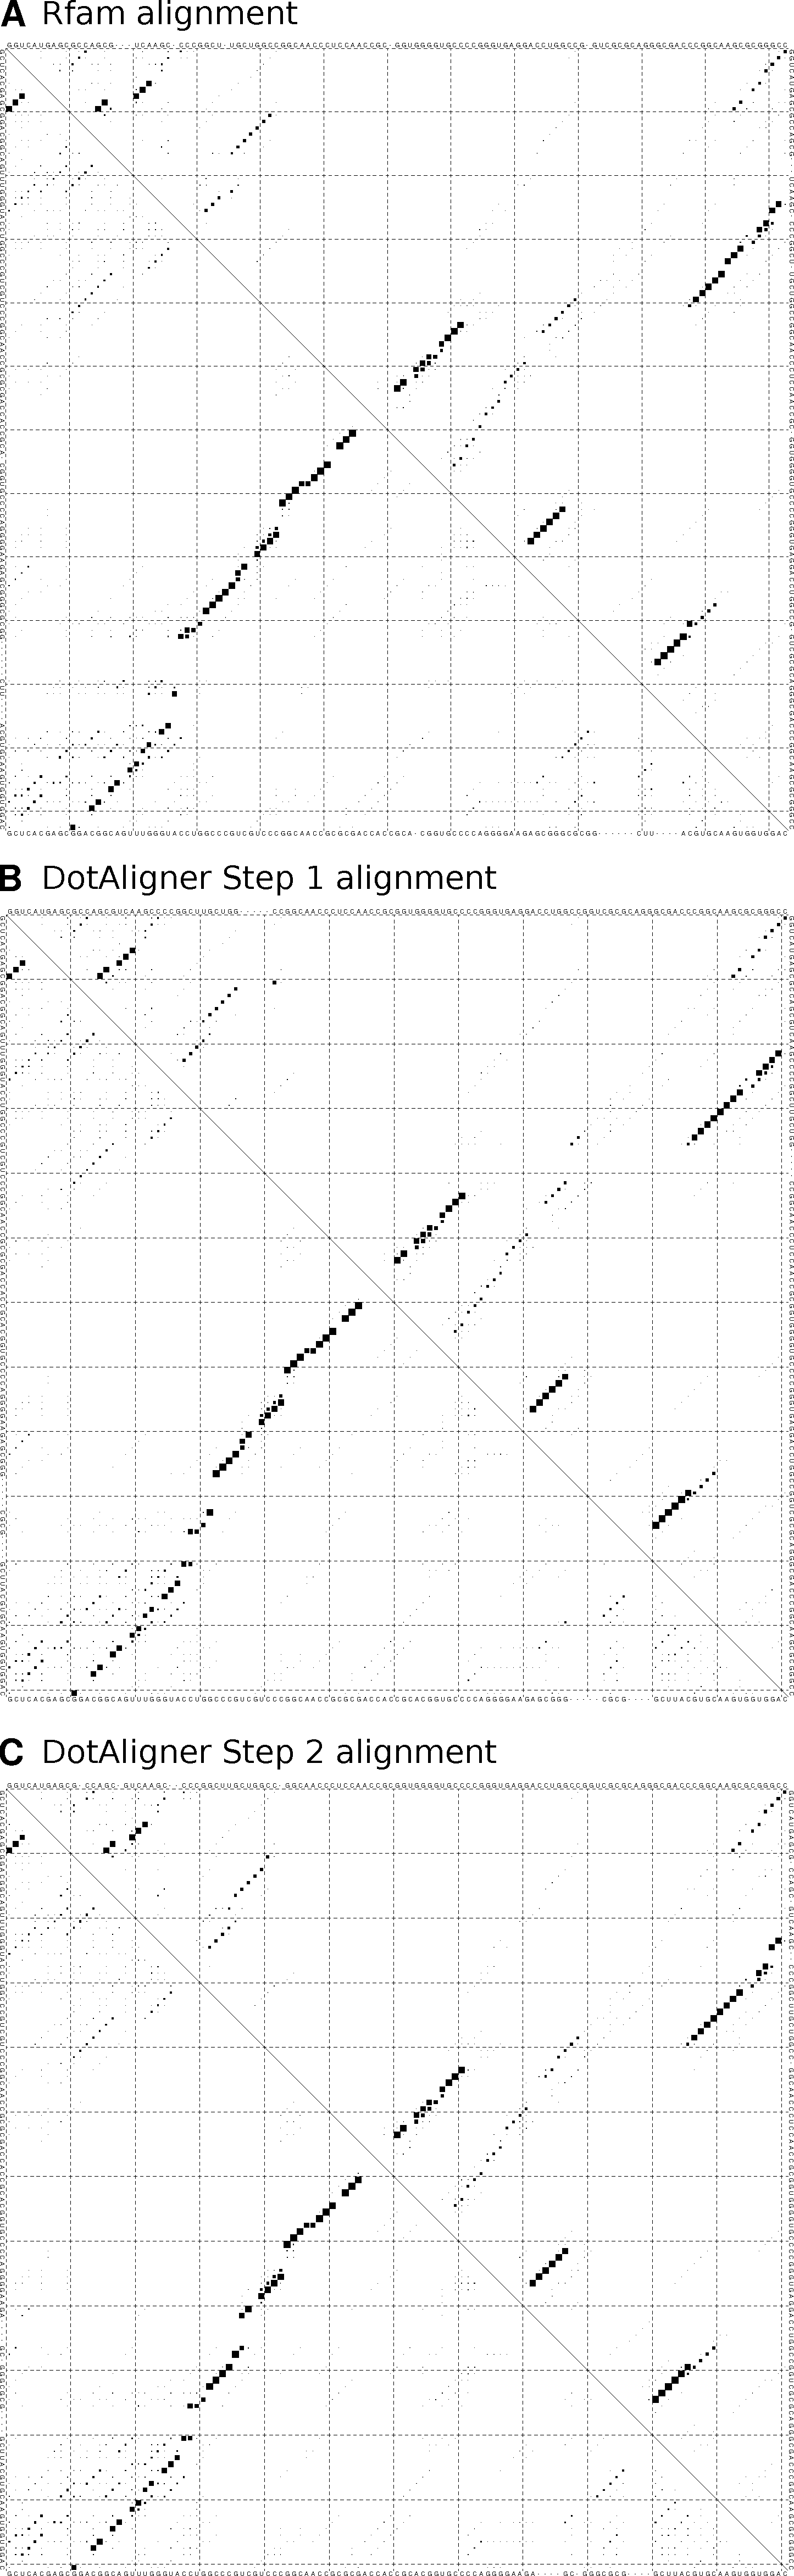
\includegraphics{SF4}
 \caption*{ \textbf{ Figure S4. Difference in sequence identity between structural and sequence alignments}\\
The difference in pairwise sequence identity for 1,189,675 randomly sampled RFAM version 12.3 seed 
 alignments is shown for sequence-only alignments using a variant of the Needleman-Wunsch algorithm
permitting free end gaps (NW) and the native RFAM seed alignments. 
Only sequences within the same family are compared, exposing the presence of  local sequence similarity within the sequences. Pairwise sequence identity is defined by the number of matching nucleotides divided by the length of the 
shortest sequence. 
}
\end{figure}

\begin{figure}
 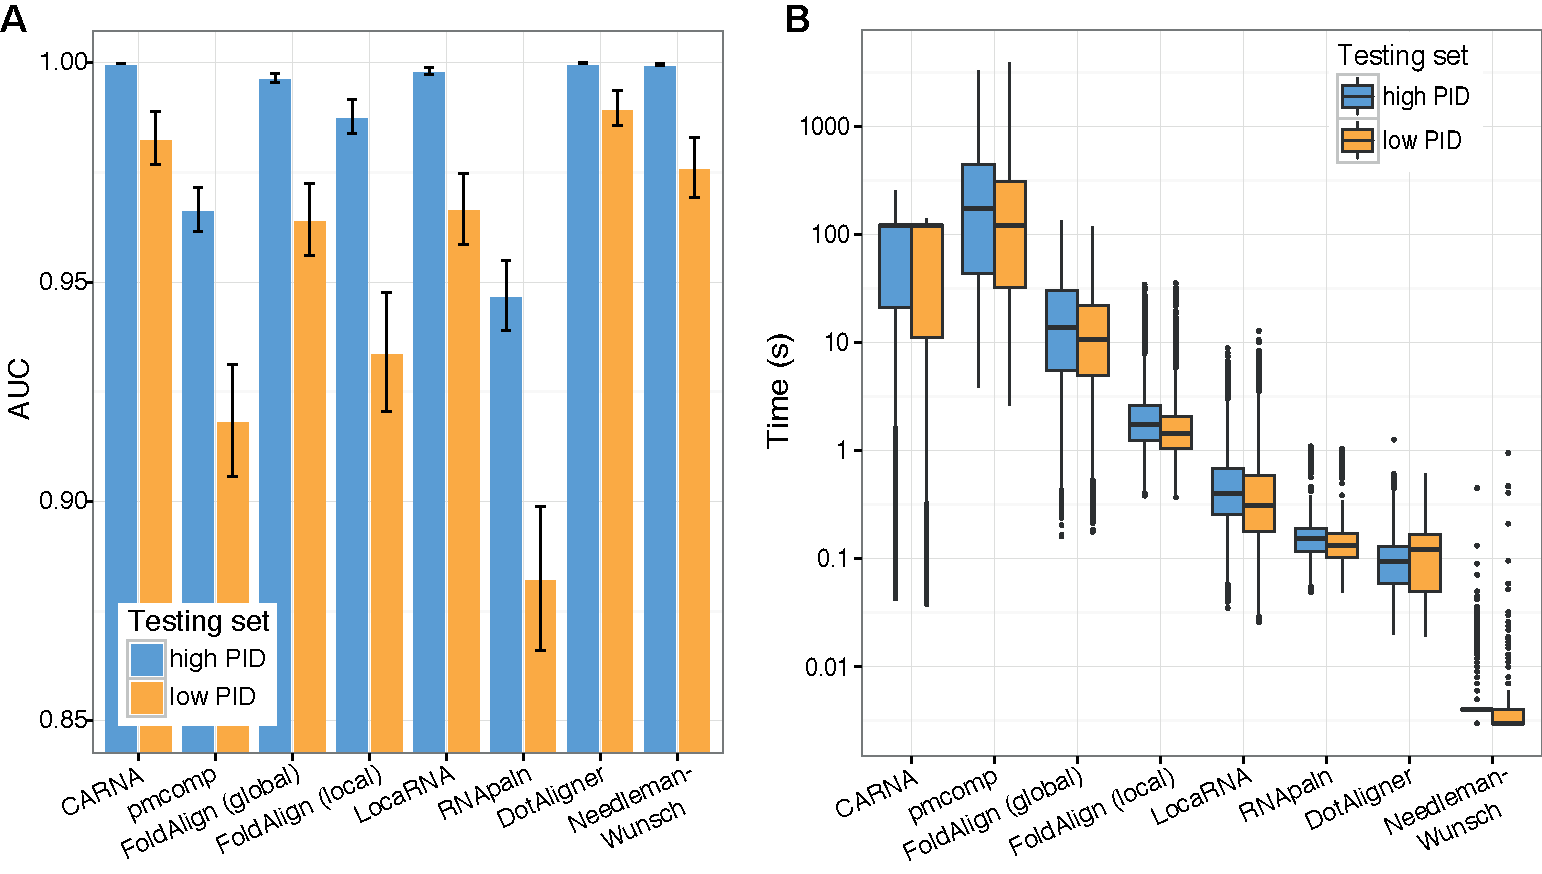
\includegraphics[width=\textwidth]{SF5}
  \caption* {{\textbf{Figure S5. Classification of known RNA structures.} }
 (\textbf{A})  Area Under the Curve (AUC) of ROC values with 95\% confidence intervals 
associated to Figure 3A. 
 (\textbf{B}) Associated runtime distribution of single thread computation on a 2.6 GHz AMD Opteron processor 
 (N.B. a fixed upper limit of 120 s was  imposed for \carna{}). } 
\end{figure}

\begin{figure}
 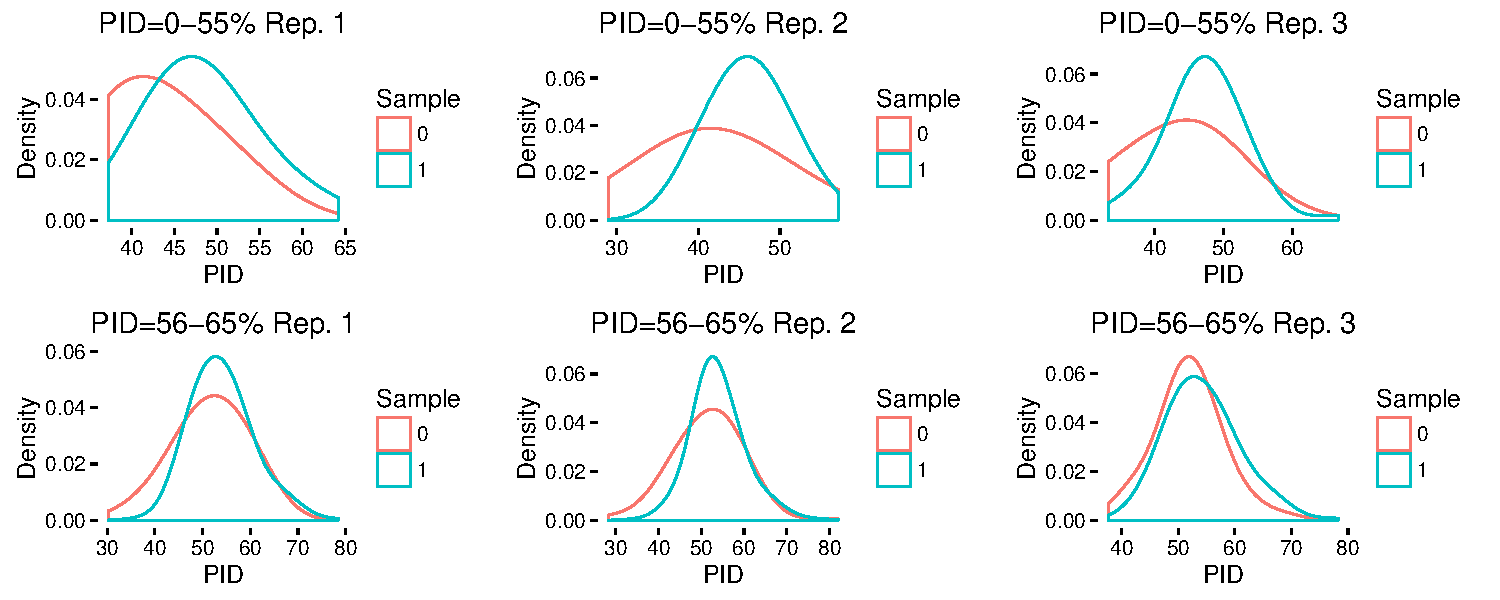
\includegraphics{SF6}
  \caption* {{\textbf{Figure S6. \dotaligner{} clustering performance in function of sequence length.} }
 (\textbf{A})  Area Under the Curve (AUC) of ROC values with 95\% confidence intervals 
for 3 replicates of stochastically sampled RFAM version 12.3 clans, controlling for sequence length (x-axis). 
N.B. the 500-1000 set only includes between 17-20 sequences given their rarity in the RFAM datasets, 
compared to 299-300 for the other samples. 
 (\textbf{B}) Associated runtime distribution of single thread computation on a 2.6 GHz AMD Opteron processor. } 
\end{figure}

%\begin{figure}
% 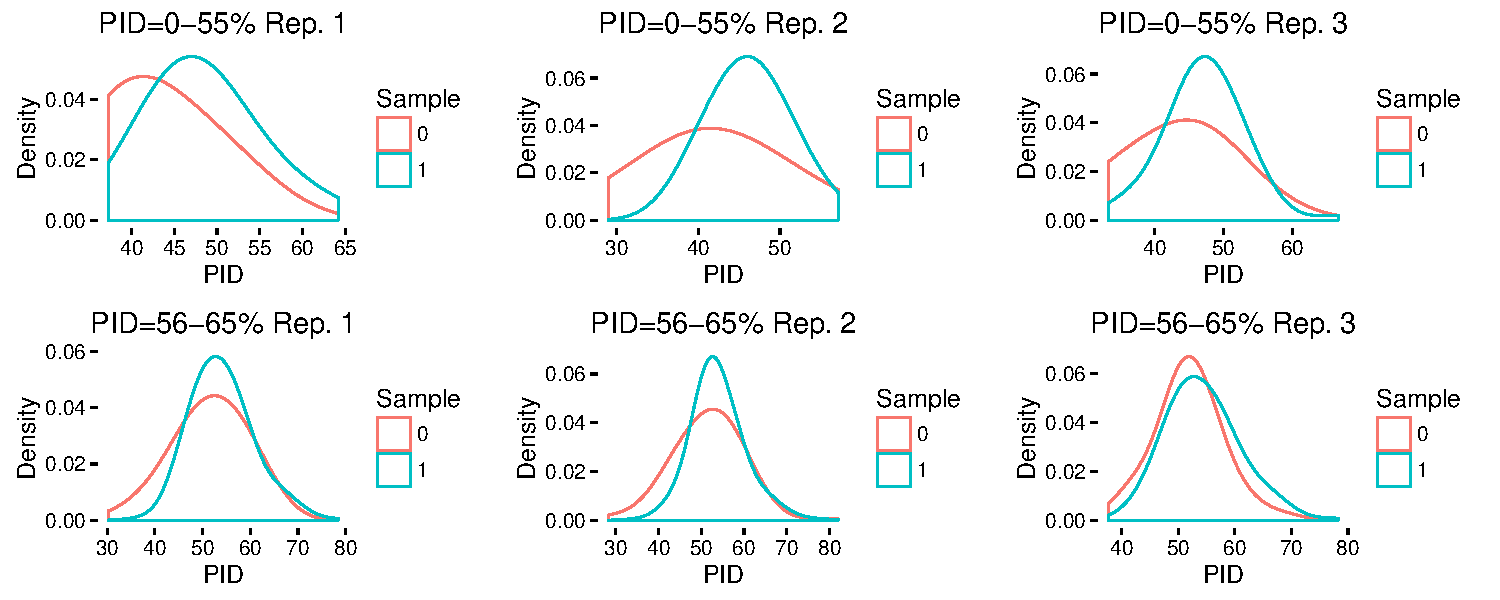
\includegraphics[width=\textwidth]{SF6}
% \caption*{ \textbf{ Figure S6. Impact of sampling of stochastic alignments on sequence identity.}\\
%The sequence identity (PID) of the \dotaligner{} predicted alignment is higher if the optimal alignment originates from the probabilistic sampling (Sample) for the benchmark dataset of low PIDs, whereas there is no difference for the benchmark dataset of medium PIDs. We executed \dotaligner{} (default runtime parameters but sampling diversity T=0.25 and number of samples s=1000) on the RFAM binary classification benchmark datasets corresponding to 0-55\% and 56-65\% sequence identity (PID) (3 replicates each). 
%}
%\end{figure}

\begin{sidewaysfigure}
 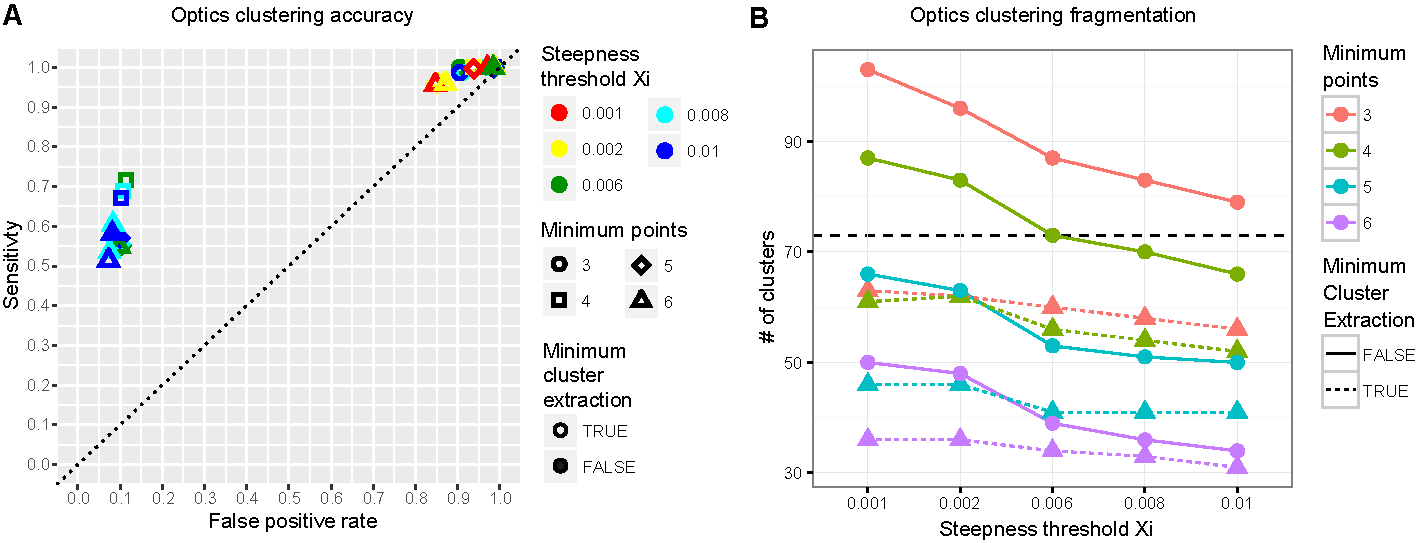
\includegraphics[width=\textwidth]{SF7}
 \caption*{ \textbf{ Figure S7. OPTICS clustering optimisation }\\
Effect of OPTICS parameters on clustering accuracy (\textbf{A}) and amount 
 of clusters (\textbf{B}) from a \dotaligner{} dissimilarity matrix of 580 reference RFAM 
 structures and their dinucleotide-shuffled controls (horizontal dashed line indicates 
 expected amount of clusters, or unique RFAM families). }
\end{sidewaysfigure}


\begin{figure}
 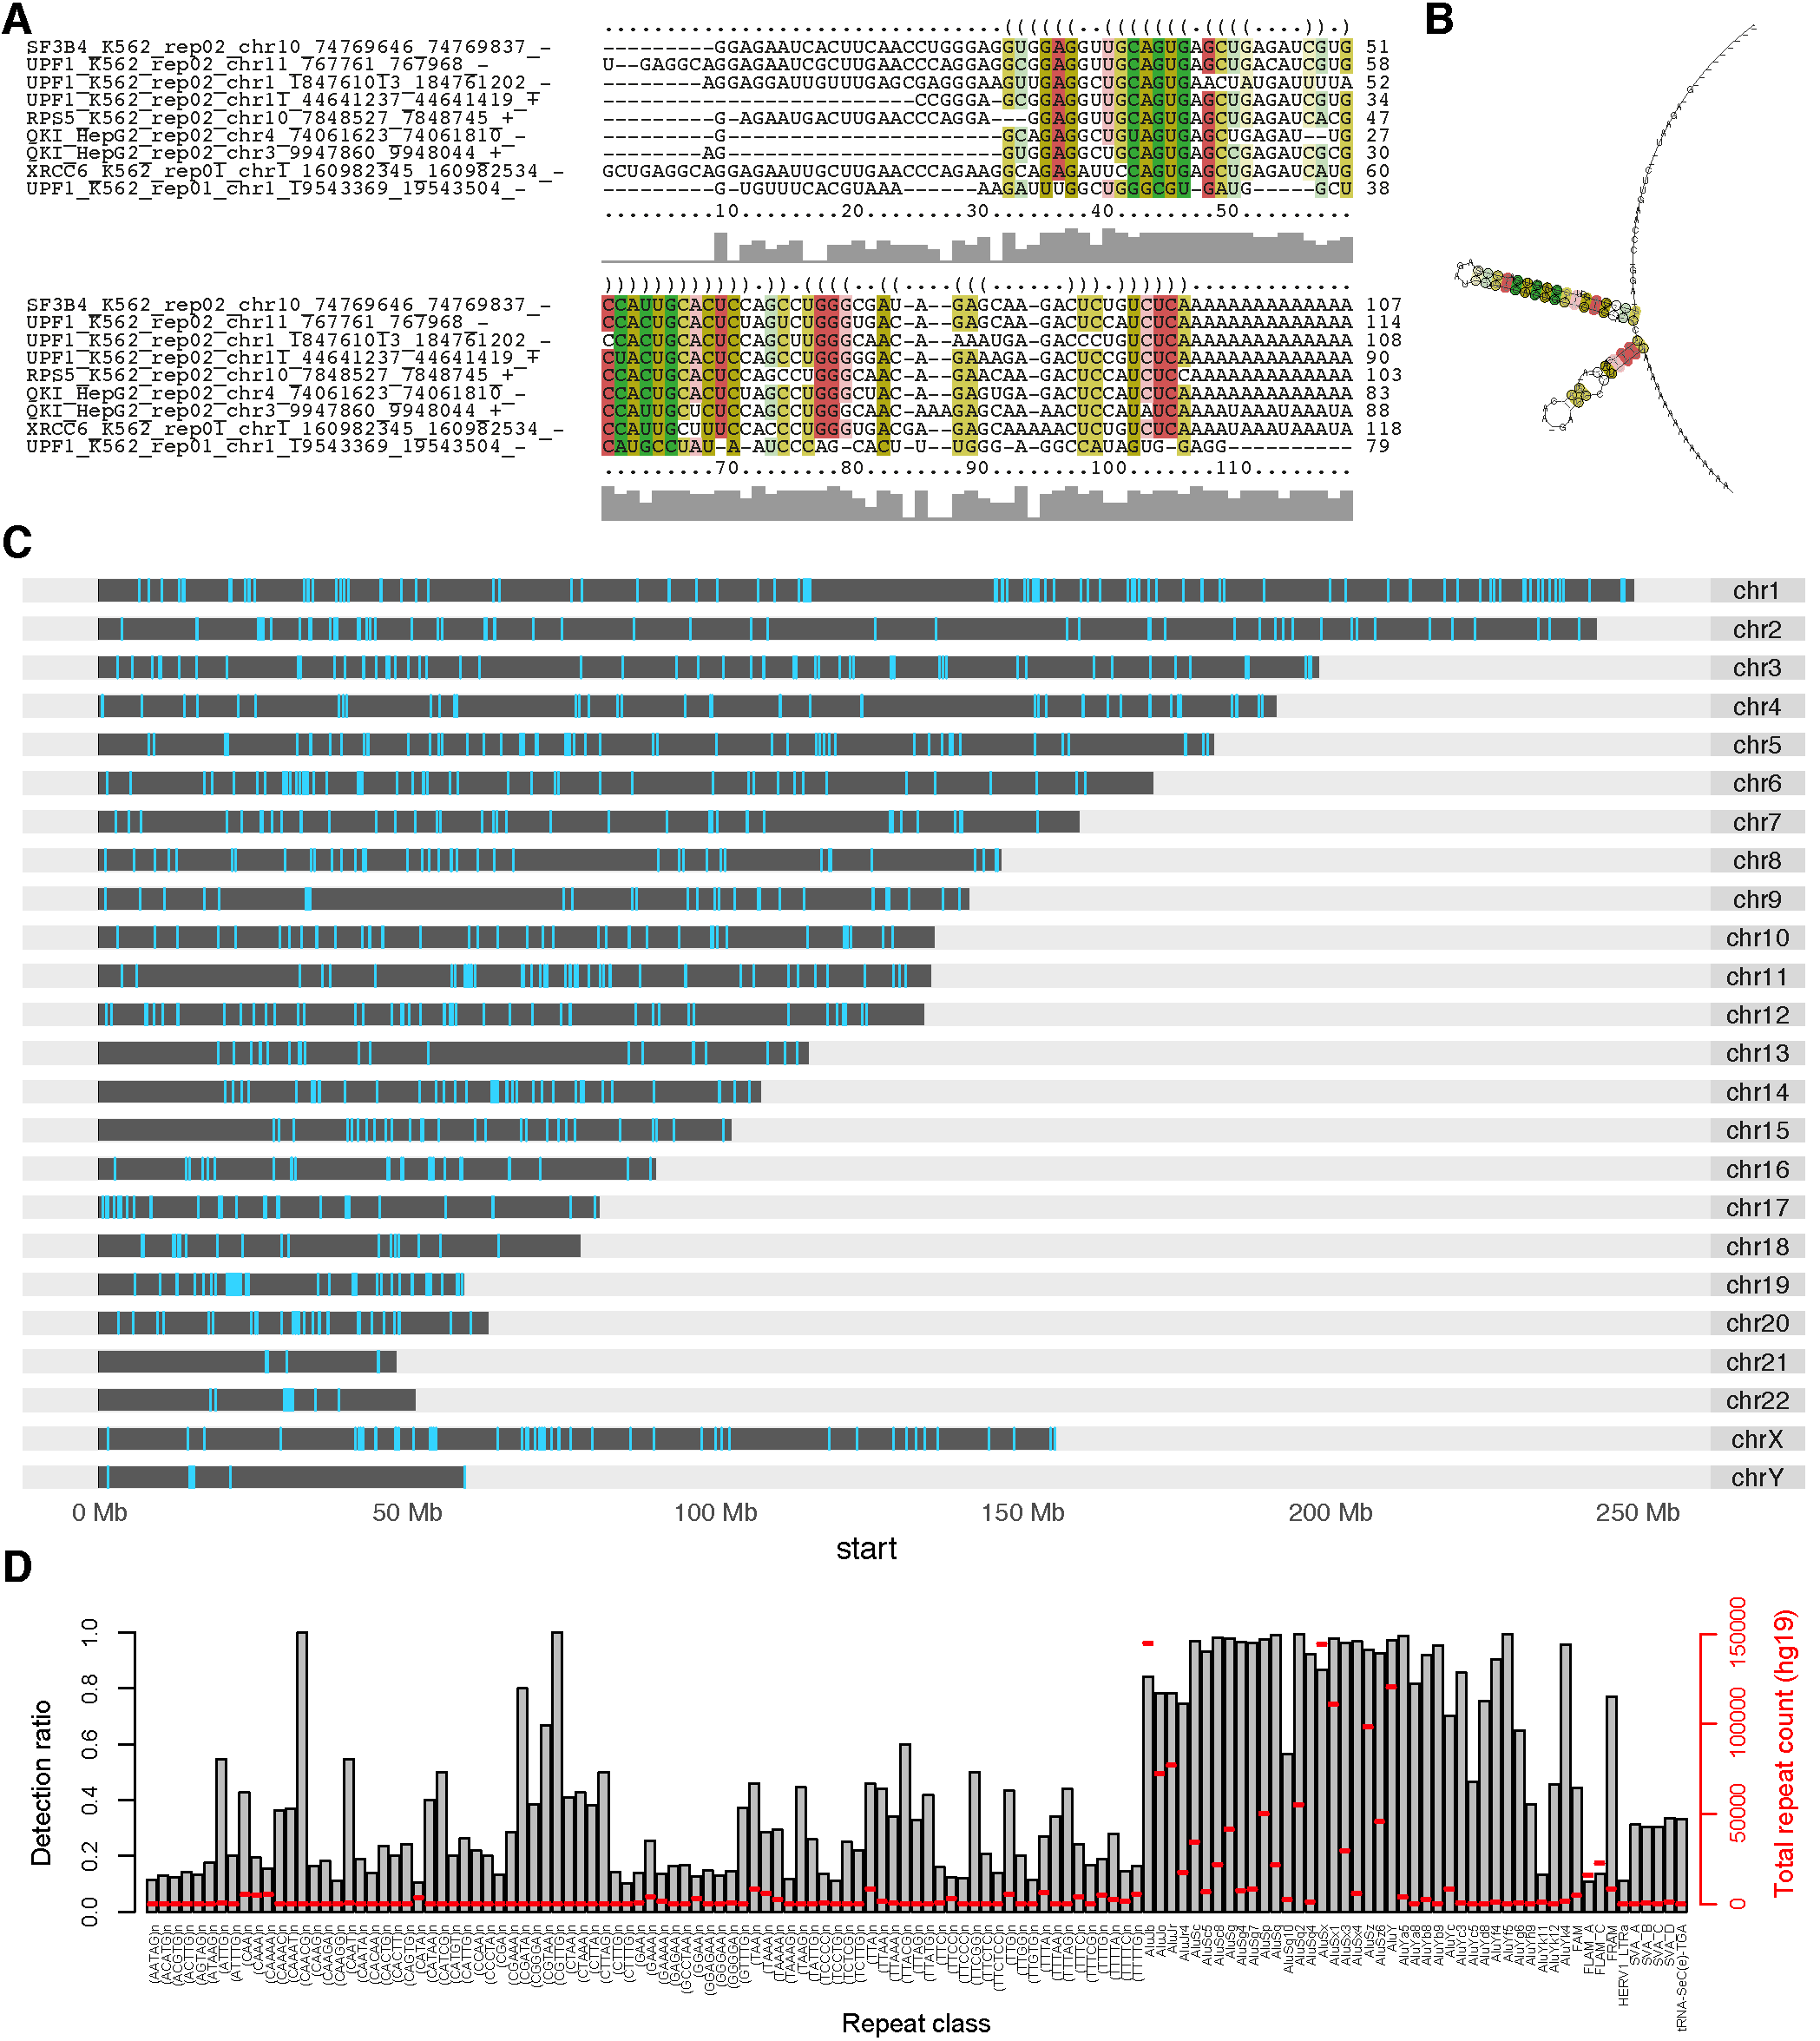
\includegraphics[width=\textwidth]{SF8}
 \caption*{ \textbf{ Figure S8. Genomic distribution of a UPF1-associated RNA structure motif }\\
(\textbf{A}) Multiple sequence alignment of a significant cluster from \textbf{Figure 5F} as produced by \texttt{mLocaRNA} and \texttt{RNAalifold}, and its associated consensus secondary structure prediction  (\textbf{B}). (\textbf{C}) Karyogram illustrating the human genomic coordinates (Grch37) of structural motif homologs, to this motif that do not overlap RepeatMasker annotations \cite{smit2010repeatmodeler}, as identified with \texttt{cmsearch }from the Infernal software package \cite{nawrocki2013infernal}. (\textbf{D}) Distribution of homologs within repeat elements (only repeats classes where $>$ 10\% of the repeats overlap homologs are displayed). 
}
\end{figure}


\end{document}
